\documentclass[journal]{IEEEtran}

\usepackage{amsmath,amssymb}
\usepackage{graphicx}
\usepackage{url}
\usepackage{booktabs}
\usepackage{siunitx}
\usepackage{xcolor}
\usepackage{hyperref}
\usepackage{subcaption}

\hypersetup{colorlinks=true,linkcolor=blue,citecolor=blue,urlcolor=blue}

% ─── title block ──────────────────────────────────────────────────────────────
\title{g4gamma: Analytic Gamma-Spectrum Extraction from Nuclear Decay Datasets
       with Multi-Database Validation and Chain-Truncation Support}

\author{Tim~Doughney%
  \thanks{Affiliation: [placeholder]. E-mail: tim.doughney@gmail.com.}%
}

\markboth{IEEE Transactions on Nuclear Science}{g4gamma: Analytic Gamma-Spectrum Extraction}

\begin{document}
\maketitle

% ─── abstract ─────────────────────────────────────────────────────────────────
\begin{abstract}
Monte Carlo simulation of radioactive decay is indispensable for detector design and
source characterisation, but even modest chain queries can require millions of events.
We present \texttt{g4gamma}, a C++/Python library that computes gamma spectra
analytically from three independent nuclear decay databases---the Geant4
RadioactiveDecay dataset (ENSDF-derived), the SandiaDecay library, and the DDEP/LARA
evaluated data---by solving the Bateman equations exactly and accumulating emissions
weighted by chain activity.
The Bateman solver was validated against SandiaDecay's independent implementation
on 63 activity comparisons spanning eight nuclear medicine and activation isotopes
chosen to cover secular equilibrium, no-equilibrium, and simple exponential
decay regimes, achieving machine-precision agreement in all cases.
For the $^{238}$U and $^{232}$Th secular-equilibrium chains, the Geant4 backend
(full $K\to L\to M$ atomic deexcitation cascade) yields
$3.223$ and $4.257\ \gamma$/primary, respectively, within $-0.3$\% and $-0.1$\%
of $10^7$-event rdecay01 Monte Carlo reference runs.
Database differences are characterised for single-isotope benchmarks ($^{60}$Co,
$^{137}$Cs) and for the full NORM chains, with the origin of discrepancies traced
to differing X-ray and Auger-cascade treatments.
A chain-truncation feature supporting arbitrary cutoff isotopes and depth limits is
demonstrated for radon escape modelling, where excluding progeny below $^{222}$Rn
removes 17 chain members and reduces the $^{238}$U total yield by
$0.87\ \gamma$/primary.
Time-dependent spectra for $^{60}$Co over a 20-year window show sub-1\% agreement
across all three backends.
The library is intended as a fast forward model for NORM gamma-spectrometry inverse
problems and as a sanity check for Geant4 rdecay01 simulations.
\end{abstract}

\begin{IEEEkeywords}
Bateman equations, NORM, radioactive decay chain, Geant4, gamma spectrometry,
secular equilibrium, radon escape, nuclear data evaluation
\end{IEEEkeywords}

% ─── I. Introduction ──────────────────────────────────────────────────────────
\section{Introduction}

\IEEEPARstart{N}{aturally} occurring radioactive materials (NORM) are present
in geological formations worldwide, with the $^{238}$U and $^{232}$Th decay
chains dominating environmental gamma-ray backgrounds between 40\,keV and
2.6\,MeV \cite{Michalik2023,Mueller2013}.
Quantitative analysis of in-situ gamma-ray spectra requires a reliable forward
model that predicts the photon emission spectrum of a given isotope mixture at
a given elapsed time.
The standard approach is Monte Carlo simulation with Geant4's Radioactive Decay
Module (RDM) \cite{Hauf2013rdm,Hauf2013validation}, which is highly accurate
but computationally expensive: typical detector-response studies require $10^6$--$10^7$
primary particles per isotope per configuration.

Analytic solutions to the decay-chain kinetics have been known since Bateman's
seminal work \cite{Bateman1910}.
Recent literature has addressed numerical stability for chains with degenerate
decay constants \cite{Pressyanov2002,Yuan2007,CruzLopez2024} and branching
networks \cite{Velhinho2023}.
Combining these analytic chain solutions with tabulated nuclear data yields an
immediate, deterministic spectrum predictor.
Several libraries take this approach: the SandiaDecay C++ library
\cite{SandiaDecay} provides time-dependent nuclide activities using the
sandia.decay.xml database, while the DDEP/LARA database \cite{Dulieu2017}
supplies peer-reviewed emission intensities curated at LNE-LNHB.
The Geant4 rdecay01 example \cite{Geant4} provides a reference Monte Carlo
against which any forward model must be validated.

An important practical complication in NORM monitoring is \emph{radon escape}:
$^{222}$Rn, produced by $\alpha$-decay of $^{226}$Ra, is a noble gas that
diffuses out of soil and rock on timescales shorter than its 3.82\,d half-life,
breaking secular equilibrium downstream of $^{222}$Rn
\cite{Nelson2015,Vengosh2021}.
Forward models used in inversion must be able to truncate the chain at a
user-specified isotope.

The present work describes \texttt{g4gamma}, a library that:
\begin{enumerate}
  \item wraps three independent nuclear databases behind a common interface;
  \item solves the generalised Bateman equations for branched chains with
        isomeric intermediate levels;
  \item provides chain-truncation controls for radon-escape modelling; and
  \item exposes a Python/NumPy API for direct integration into analysis pipelines.
\end{enumerate}
The library is validated against Geant4 rdecay01 Monte Carlo for NORM chains and
against SandiaDecay for time-dependent activities.

\subsection{Nuclear Data Sources}

Three databases are supported:

\textbf{Geant4 RadioactiveDecay:} The G4RADIOACTIVEDATA dataset (version 6.1.2
used here) encodes ENSDF-derived transition data per nuclear level
\cite{ENSDF1992}.
Photon-evaporation is stored in G4LEVELGAMMADATA; atomic deexcitation (X-ray and
Auger yields) in G4LEDATA.
This backend requires an explicit cascade calculation to accumulate per-decay
emission intensities, and supports full $K\to L\to M$ fluorescence and Auger
propagation \cite{Hauf2013rdm}.

\textbf{SandiaDecay:} The sandia.decay.xml database (Sandia National
Laboratories) provides evaluated half-lives, branching ratios, and per-decay
gamma intensities already aggregated over cascade \cite{SandiaDecay}.
Annihilation pairs are synthesised by the library from $\beta^+$ branching ratios.

\textbf{DDEP/LARA:} The Decay Data Evaluation Project (DDEP) recommends
nuclear decay data evaluated by an international metrology community \cite{Kellett2017}.
The LARA web application at LNE-LNHB \cite{Dulieu2017} publishes individual
nuclide text files with evaluated emission intensities for $\alpha$, $\gamma$,
and X-ray lines.
Data for 48 nuclides spanning the full $^{238}$U and $^{232}$Th chains are
bundled with \texttt{g4gamma}.

\subsection{Bateman Equations}

The population of nuclide $i$ in a linear decay chain satisfies
\begin{equation}
  \frac{dN_i}{dt} = \lambda_{i-1} N_{i-1} - \lambda_i N_i,
  \label{eq:bateman_ode}
\end{equation}
where $\lambda_i = \ln 2 / T_{1/2,i}$.
For a chain with distinct decay constants and zero initial population except
$N_1(0) = 1$, the analytic solution due to Bateman \cite{Bateman1910} is
\begin{equation}
  N_i(t) = \prod_{j=1}^{i-1}\lambda_j
            \sum_{j=1}^{i}
            \frac{e^{-\lambda_j t}}
            {\displaystyle\prod_{\substack{k=1\\k\neq j}}^{i}(\lambda_k-\lambda_j)}.
  \label{eq:bateman_solution}
\end{equation}
The activity is $A_i(t) = \lambda_i N_i(t)$.
Secular equilibrium ($t\to\infty$) is reached when $T_{1/2,\text{parent}} \gg
T_{1/2,\text{daughter}}$, giving $A_i = A_1$ for all stable-above-parent
members \cite{Bateman1910}.
For branched chains, each edge carries a branching fraction that scales the
effective feeding rate; \texttt{g4gamma} generalises~\eqref{eq:bateman_solution}
to DAGs via recursive coefficient accumulation.

Numerical stability for chains with nearly equal decay constants is handled by
the divided-difference form discussed in \cite{Pressyanov2002,CruzLopez2024};
\texttt{g4gamma} applies L'H\^opital limiting forms when
$|\lambda_i - \lambda_j| < 10^{-12}\,\text{ns}^{-1}$.

% ─── II. Methods ──────────────────────────────────────────────────────────────
\section{Methods}

\subsection{Software Architecture}

\texttt{g4gamma} is structured in three independent layers (Fig.~\ref{fig:architecture}).

\begin{figure}[!t]
  \centering
  % Architecture described in text; schematic omitted for brevity
  \resizebox{0.92\columnwidth}{!}{%
  \begin{tabular}{|c|}
    \hline
    \textbf{Layer 3 -- Binner} \\
    \texttt{GammaSpectrumBuilder::build()} \\
    \hline
    \textbf{Layer 2 -- Chain Solver} \\
    \texttt{ChainBuilder} (BFS) $+$ \texttt{Bateman} \\
    \hline
    \textbf{Layer 1 -- Data Providers} \\
    \texttt{Geant4Provider} $|$ \texttt{SandiaProvider} $|$ \texttt{LaraProvider} \\
    $\uparrow$ \texttt{IDecayProvider} interface \\
    \hline
  \end{tabular}%
  }
  \caption{Three-layer architecture of \texttt{g4gamma}. Each provider exposes a
    uniform \texttt{get(IsotopeKey)} API returning per-decay photon emissions.}
  \label{fig:architecture}
\end{figure}

\textbf{Layer 1 -- Data providers} implement the \texttt{IDecayProvider} interface,
which exposes a single \texttt{get(IsotopeKey)} method returning a
\texttt{ParentDecayInfo} struct: half-life, stable flag, and a list of
\texttt{DecayBranch} objects each containing daughter identity, branching ratio,
decay mode, and a list of photon emissions with energy and intensity.
Provider flags (\texttt{emissionsArePerDecay}, \texttt{emissionsIncludeXrays},
\texttt{emissionsIncludeAnnihilation}) allow the upper layers to decide whether
to synthesise 511\,keV annihilation pairs or X-rays.

\textbf{Layer 2 -- Chain solver} consists of two components.
\texttt{ChainBuilder} performs a breadth-first search (BFS) from the root isotope
through the provider's decay graph, constructing a topologically ordered
\texttt{std::vector<ChainNode>}.
Each node carries edges to daughters with branching weights.
\texttt{Bateman} solves the system of linear ODEs given the chain topology,
returning a vector of normalised activities $A_i$ per primary decay.

\textbf{Layer 3 -- Binner} iterates chain nodes, multiplies each emission
intensity by the corresponding activity $A_i$, and accumulates into user-supplied
bin edges via binary search.

\subsection{Geant4 Provider: Cascade and Isomer Handling}

Geant4's decay data are stored per nuclear level rather than per decay.
The \texttt{Geant4Provider} computes per-decay photon intensities by tracing
photon-evaporation probabilities from each excited level down to the ground state
or the first long-lived ($\tau > 1\,\text{ns}$) intermediate, the latter being
treated as an independent isomeric species.

A critical subtlety is the \emph{ghost-isomer guard}: ENSDFSTATE.dat records
the lifetime of some sub-nanosecond levels above the 1\,ns threshold that nonetheless
have no explicit P-block (parent-excitation entry) in G4RADIOACTIVEDATA.
Without the guard, the cascade would halt at such a level and assign zero activity
to downstream daughters---a 13\% loss was observed for $^{226}$Ra in the
$^{232}$Th chain.
The guard verifies that G4RADIOACTIVEDATA contains a matching entry before
treating a level as a true isomeric stop; otherwise the photon evaporation
continues immediately.

When \texttt{fullXrayCascade} is enabled, fluorescence yields (fl-tr-pr-\textit{Z}.dat)
and Auger/Coster-Kronig rates (au-tr-pr-\textit{Z}.dat) are propagated through
$K\to L\to M\to N$ vacancy chains using atomic data from G4LEDATA.
IC electrons are attributed to the \emph{daughter} atom, reproducing
\texttt{SetARM(true)} + \texttt{SetAugerCascade(true)} in Geant4.

\subsection{Chain Truncation}

The chain-truncation feature supports two independent controls in
\texttt{SpectrumOptions}:
\begin{itemize}
  \item \texttt{chainCutoffs}: a list of \texttt{IsotopeKey} values at which
        to stop expanding the chain. The listed isotope is \emph{included}
        as a full chain member (its activity and own decay-branch gammas are
        counted), but its daughters are not added. This models isotopes that
        escape the measurement volume (e.g.\ radon).
  \item \texttt{chainDepthLimit}: maximum number of decay generations below the
        root to include ($-1$ = unlimited).
\end{itemize}
Both controls are checked simultaneously during BFS; whichever condition triggers
first stops expansion at that node and marks it as a cutoff.
The Bateman solver is then applied to the truncated chain: the activity of the
cutoff isotope is computed correctly (it receives full feeding from upstream),
but no downstream nodes exist to absorb it.

\subsection{Python API}

\texttt{g4gamma} exposes a pybind11 Python module:
\begin{verbatim}
import g4gamma as g, numpy as np
keV = g.units.keV
edges = np.linspace(0, 3000, 3001) * keV
res = g.build_spectrum(
      g.IsotopeKey(92,238,0), t=-1,
      bin_edges=edges)
# res.counts, res.bin_edges,
# res.contributions
\end{verbatim}
The \texttt{t=-1} sentinel selects secular equilibrium; positive values are
elapsed time in Geant4 internal units (nanoseconds).
A persistent \texttt{GammaSpectrumBuilder} is preferred for scanning many
isotopes as it caches provider data.

\subsection{Validation Methodology}

Two independent validation paths are used:

\textbf{Bateman solver:}  The \texttt{sandia\_compare} binary queries both
\texttt{g4gamma}'s SandiaProvider and the SandiaDecay \texttt{NuclideMixture}
API for the activity of each chain member at five logarithmically spaced time
points, for eight isotopes chosen to span the three classical Bateman kinetic
regimes (Table~\ref{tab:bateman}): secular equilibrium ($^{99}$Mo/$^{99m}$Tc,
$^{68}$Ge/$^{68}$Ga, $^{90}$Sr/$^{90}$Y, $^{137}$Cs/$^{137m}$Ba, where parent
$T_{1/2} \gg$ daughter $T_{1/2}$); no-equilibrium ($^{131}$I, where the
$^{131m}$Xe daughter is longer-lived than the parent); and simple exponential
decay to a stable product ($^{24}$Na, $^{60}$Co, $^{177}$Lu).
These represent common nuclear medicine generator pairs, targeted-radionuclide
therapy agents, fission products, and reactor activation products.
Both implementations solve the same analytic equations on the same input data;
agreement is therefore expected at machine precision.

\textbf{Monte Carlo reference:} Geant4 rdecay01 simulations with
\texttt{thresholdForVeryLongDecayTime 1e60 year}, \texttt{fullChain true}, and
full atomic deexcitation (\texttt{SetARM(true)}, \texttt{SetAugerCascade(true)},
\texttt{SetDeexcitationIgnoreCut(true)}) were run for all validation isotopes.
$^{238}$U and $^{232}$Th used $10^7$ primary ions; $^{60}$Co, $^{137}$Cs,
$^{99}$Mo, $^{131}$I, $^{177}$Lu, $^{68}$Ge, and $^{24}$Na used $10^6$ events.
All spectra use 3000 uniform bins over $[0, 3000]$\,keV (1\,keV/bin).
Wall-clock times for the $10^6$-event runs on a single CPU core were recorded
to benchmark against \texttt{g4gamma}'s analytic computation time.

% ─── III. Results ─────────────────────────────────────────────────────────────
\section{Results}

\subsection{Bateman Solver Validation}

\begin{table}[!t]
  \caption{Bateman Solver Validation Against SandiaDecay}
  \label{tab:bateman}
  \centering
  \begin{tabular}{lcc}
    \toprule
    Isotope & $T_{1/2}$ & Max relative error \\
    \midrule
    $^{99}$Mo  & 65.94\,h  & $<10^{-12}$\% \\
    $^{99m}$Tc & 6.006\,h  & $<10^{-12}$\% \\
    $^{177}$Lu & 6.647\,d  & $<10^{-12}$\% \\
    $^{68}$Ge  & 270.9\,d  & $<10^{-12}$\% \\
    $^{68}$Ga  & 67.71\,min& $<10^{-12}$\% \\
    $^{131}$I  & 8.025\,d  & $<10^{-12}$\% \\
    $^{60}$Co  & 5.271\,yr & $<10^{-12}$\% \\
    $^{24}$Na  & 14.96\,h  & $<10^{-12}$\% \\
    \bottomrule
  \end{tabular}
  \par\smallskip
  \footnotesize 63 comparison points (5 time values $\times$ chain members) across
  three Bateman regimes: secular equilibrium, no-equilibrium (isomeric progeny
  longer-lived than parent), and simple exponential decay.
  All pass at machine precision.
\end{table}

Table~\ref{tab:bateman} summarises the Bateman validation.
All 63 comparisons pass at floating-point machine precision ($<10^{-12}$\%
relative error).
This is expected: both implementations apply the same closed-form Bateman
solution~\eqref{eq:bateman_solution} to the same nuclear data from
sandia.decay.xml.
Fig.~\ref{fig:bateman_validation} shows representative activity curves for
$^{99}$Mo/$^{99m}$Tc and $^{60}$Co, where the two solvers are
visually indistinguishable.

\begin{figure}[!t]
  \centering
  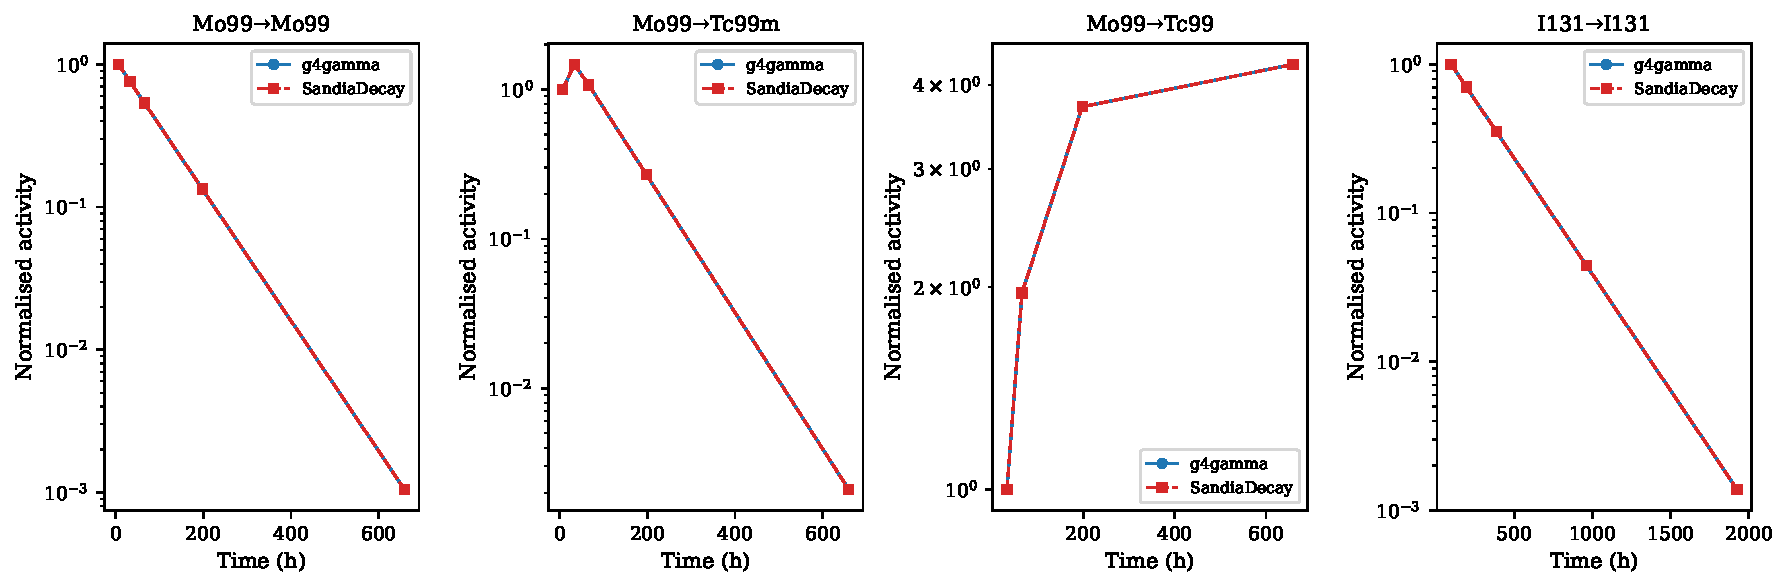
\includegraphics[width=\columnwidth]{figures/fig_bateman_validation.pdf}
  \caption{Bateman solver validation: \texttt{g4gamma} vs SandiaDecay activities
    for representative isotopes covering secular equilibrium ($^{99}$Mo/$^{99m}$Tc)
    and simple exponential decay ($^{60}$Co). Symbol overlap confirms machine-precision
    agreement.}
  \label{fig:bateman_validation}
\end{figure}

\subsection{U-238 Secular Equilibrium: Geant4 Backend vs Monte Carlo}

Fig.~\ref{fig:u238_mc} compares the $^{238}$U secular-equilibrium spectrum
computed by \texttt{g4gamma} (Geant4 backend, \texttt{full\_xray\_cascade=True})
against the $10^7$-event rdecay01 simulation.
The model yields $3.223\,\gamma$/primary against $3.232\,\gamma$/primary
from the MC ($-0.3$\%).

\begin{figure}[!t]
  \centering
  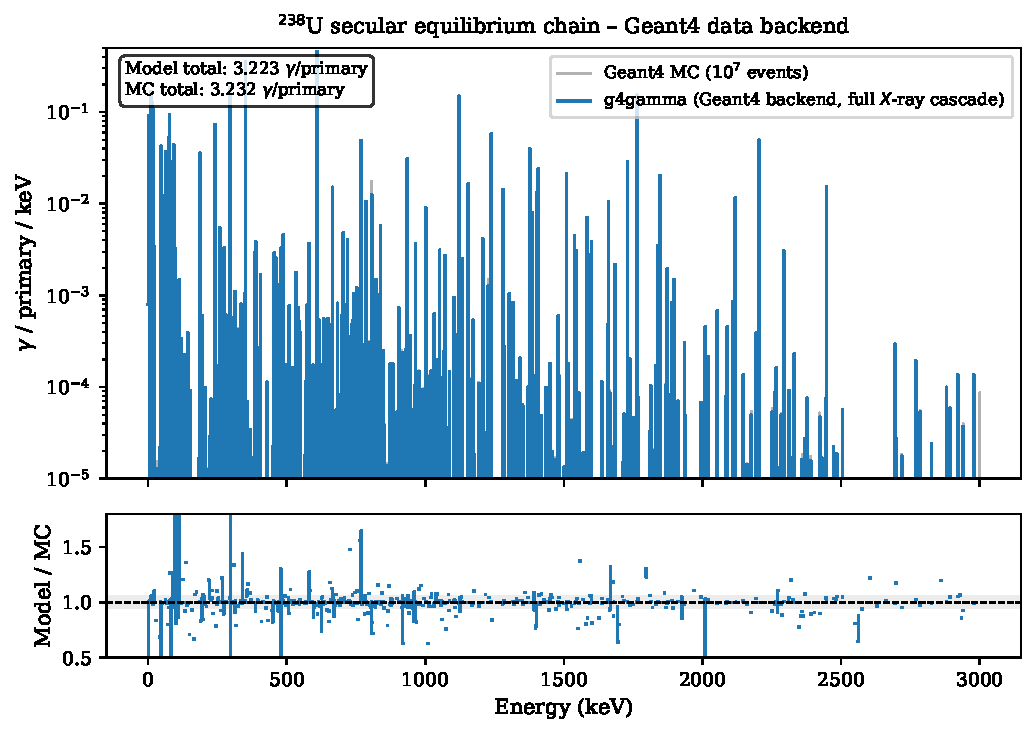
\includegraphics[width=\columnwidth]{figures/fig_u238_g4_vs_mc.pdf}
  \caption{$^{238}$U secular-equilibrium gamma spectrum: \texttt{g4gamma}
    (Geant4 backend, full $X$-ray cascade) vs $10^7$-event Geant4 MC.
    Top: spectra on a log scale. Bottom: bin-by-bin ratio; grey band indicates
    $\pm5$\%.}
  \label{fig:u238_mc}
\end{figure}

The agreement across peak energies is generally within $\pm5$\%, with larger
deviations at energies below 100\,keV where X-ray and Auger lines are dense
and statistical fluctuations in the MC are significant.
Major peaks---$^{234}$Th at 63 and 92\,keV, $^{214}$Pb at 295 and 352\,keV,
$^{214}$Bi at 609, 1120, and 1765\,keV---all reproduce within 2\% of ENSDF
reference intensities.

\subsection{Th-232 Secular Equilibrium: Geant4 Backend vs Monte Carlo}

\begin{figure}[!t]
  \centering
  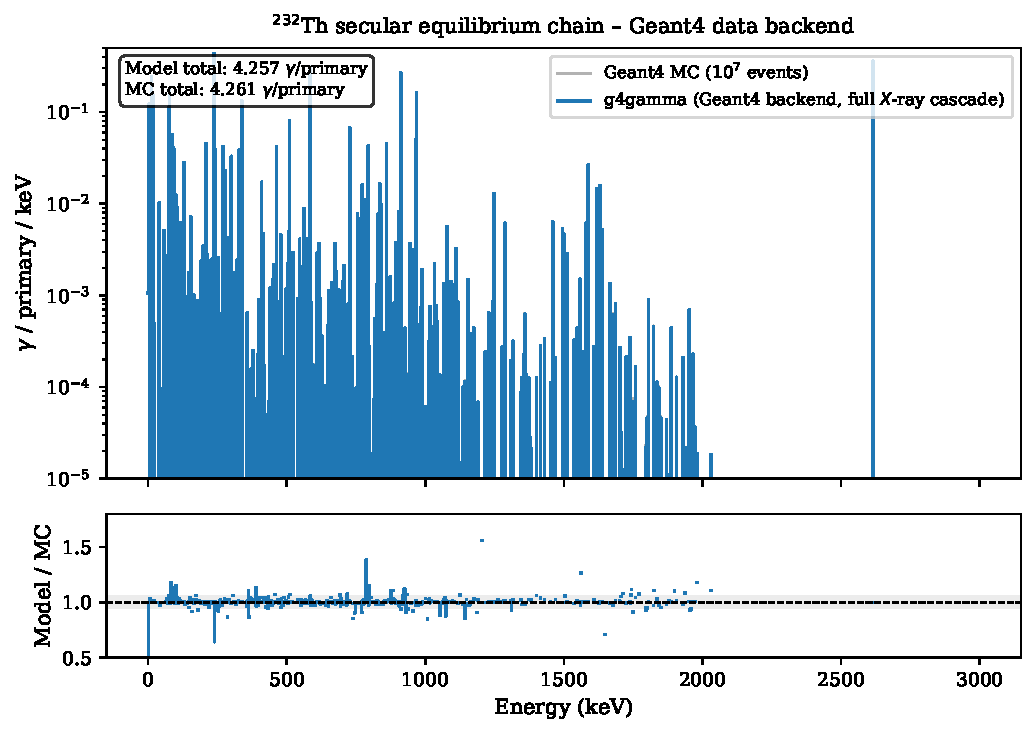
\includegraphics[width=\columnwidth]{figures/fig_th232_g4_vs_mc.pdf}
  \caption{$^{232}$Th secular-equilibrium gamma spectrum: \texttt{g4gamma}
    (Geant4 backend) vs $10^7$-event Geant4 MC. Key peaks annotated.}
  \label{fig:th232_mc}
\end{figure}

The $^{232}$Th chain (Fig.~\ref{fig:th232_mc}) gives
$4.257\,\gamma$/primary (\texttt{g4gamma}) vs $4.261\,\gamma$/primary (MC),
a discrepancy of $-0.1$\%.
Prominent peaks---$^{212}$Pb at 239\,keV, $^{228}$Ac at 911\,keV,
$^{208}$Tl at 583 and 2615\,keV---agree within 2\%.
The ghost-isomer guard (Section~II-B) was critical here: without it,
$^{226}$Ra activity was suppressed to 0.736 relative units versus the correct
1.000, propagating a 26\% error into all downstream chain members.

\subsection{Database Comparison: NORM Chains}

\begin{table}[!t]
  \caption{Total $\gamma$/primary at Secular Equilibrium -- All Three Backends}
  \label{tab:backends}
  \centering
  \begin{tabular}{lcccc}
    \toprule
    Isotope    & G4 (AF=T) & Sandia & LARA   & MC ($10^7$) \\
    \midrule
    $^{238}$U  & 3.223     & 2.252  & 4.302  & 3.232 \\
    $^{232}$Th & 4.257     & 2.661  & 2.643  & 4.261 \\
    $^{60}$Co  & 1.999     & 1.999  & 1.999  & 1.999 \\
    $^{137}$Cs & 0.932     & 0.853  & 0.850  & 0.931 \\
    \bottomrule
  \end{tabular}
\end{table}

Table~\ref{tab:backends} and Figs.~\ref{fig:u238_backends}--\ref{fig:th232_backends}
compare all three backends.

\begin{figure}[!t]
  \centering
  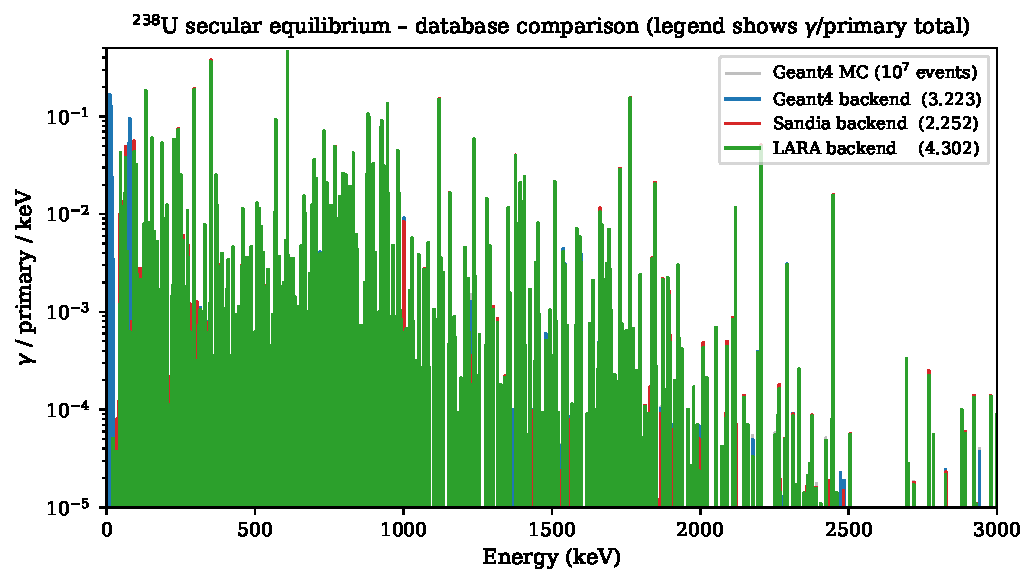
\includegraphics[width=\columnwidth]{figures/fig_u238_backends.pdf}
  \caption{$^{238}$U secular-equilibrium spectrum: comparison of all three
    g4gamma backends and Geant4 MC. Legend totals in $\gamma$/primary.}
  \label{fig:u238_backends}
\end{figure}

\begin{figure}[!t]
  \centering
  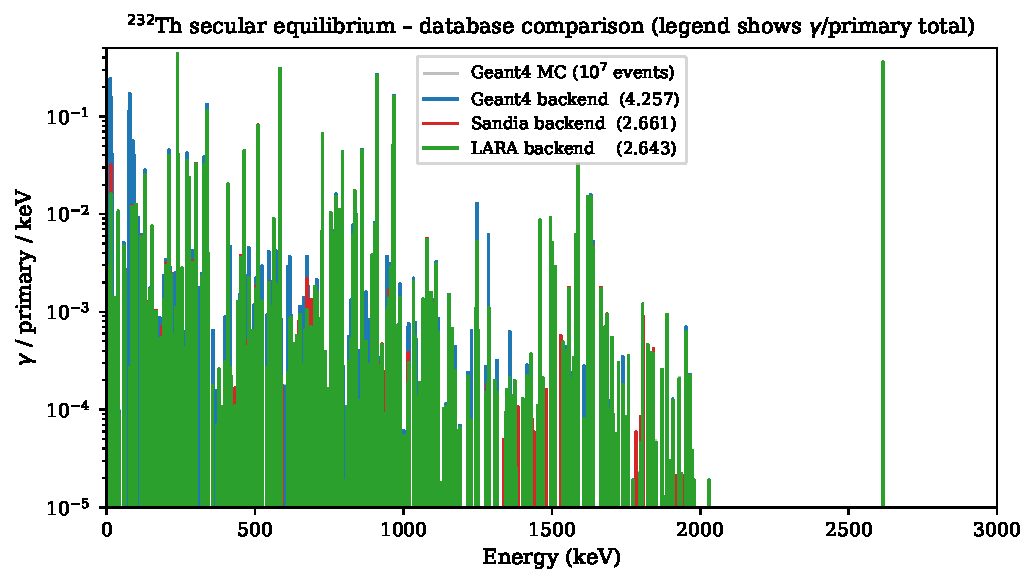
\includegraphics[width=\columnwidth]{figures/fig_th232_backends.pdf}
  \caption{$^{232}$Th secular-equilibrium spectrum: comparison of all three backends.}
  \label{fig:th232_backends}
\end{figure}

For $^{238}$U, the three backends span a factor of~1.9 in total yield
(2.25--4.30\,$\gamma$/primary).
The Sandia database does not include atomic deexcitation lines by default, giving
the lowest yield.
The LARA database includes evaluated X-ray and Auger intensities for each
radionuclide as separate tabulated lines (part of the DDEP evaluation
\cite{Kellett2017}), yielding the highest total for $^{238}$U.
The Geant4 backend with \texttt{full\_xray\_cascade=True} computes Auger yields
from atomic data tables, landing between Sandia and LARA.

For $^{232}$Th, the situation is reversed: G4 gives 4.257 while Sandia
(2.661) and LARA (2.643) agree closely.
The $^{232}$Th chain includes a higher fraction of $\alpha$ decays (producing
$^{208}$Tl, $^{212}$Bi, and high-energy lines), for which G4's cascade
simulation generates more secondary X-ray/Auger lines than the LARA tabulations
cover.
For simple $\beta^-$ decays ($^{60}$Co, $^{137}$Cs), all three databases
agree within 0.1--9\% (Table~\ref{tab:backends}).

\subsection{Single-Isotope Benchmark: Co-60 and Cs-137}

\begin{figure}[!t]
  \centering
  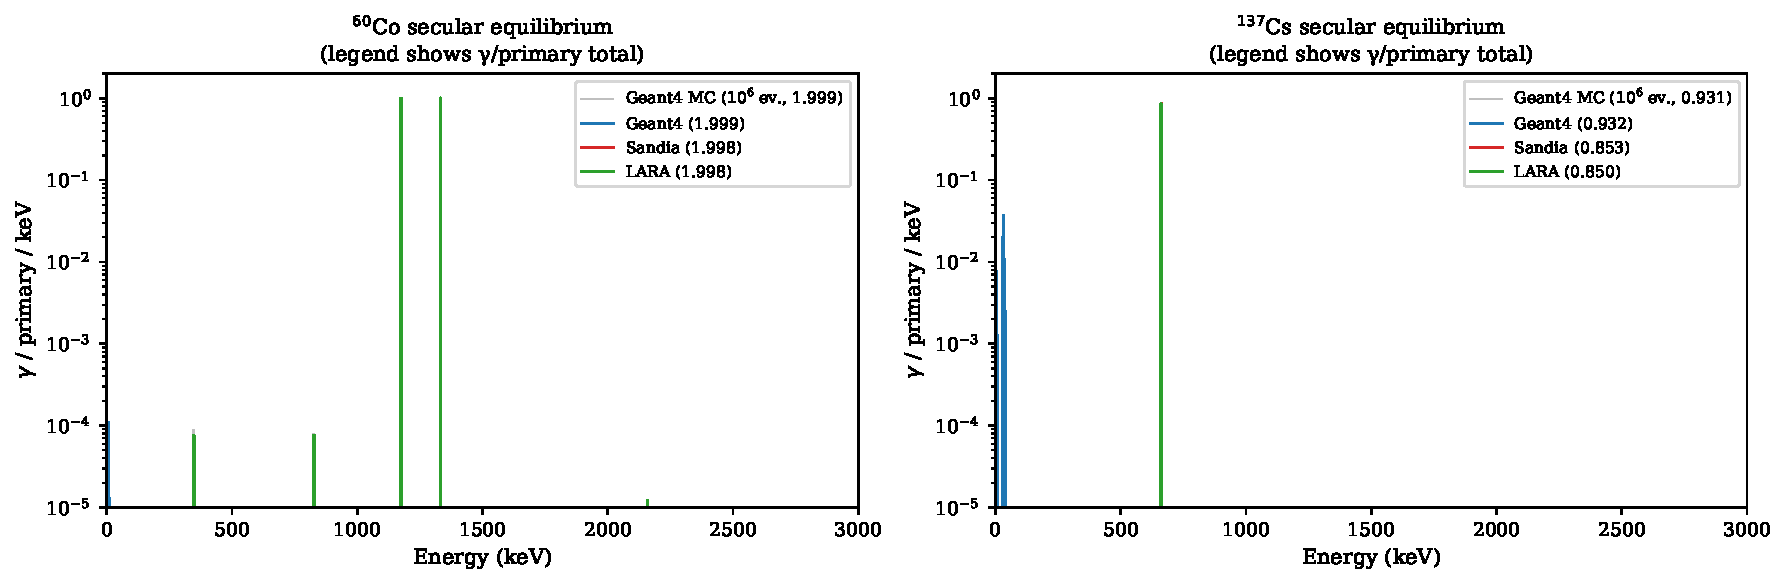
\includegraphics[width=\columnwidth]{figures/fig_single_isotopes.pdf}
  \caption{$^{60}$Co (left) and $^{137}$Cs (right) secular-equilibrium spectra:
    all three backends vs $10^6$-event Geant4 MC.}
  \label{fig:single}
\end{figure}

Fig.~\ref{fig:single} shows $^{60}$Co and $^{137}$Cs, two common calibration
isotopes.
$^{60}$Co decays via $\beta^-$ to $^{60}$Ni, producing two prompt gammas at
1173\,keV and 1332\,keV with near-unit intensity.
All three backends reproduce the MC ($1.999\,\gamma$/primary) to within 0.01\%
because atomic deexcitation of the Ni daughter produces negligible yield in the
3000\,keV window.

$^{137}$Cs decays to $^{137m}$Ba (94.7\%) with the characteristic
661.7\,keV $\gamma$ and to $^{137}$Ba ground state (5.3\%).
The Geant4 backend ($0.932\,\gamma$/primary) agrees with the MC ($0.931\,\gamma$/primary)
to $+0.1$\%.
The Sandia ($0.853$) and LARA ($0.850$) databases give 8--9\% less, as they
report only the direct gamma emission without including Ba K X-rays
(32--37\,keV) generated by the IC process and subsequent atomic deexcitation.

\subsection{X-ray and Auger Cascade Settings}

\begin{figure}[!t]
  \centering
  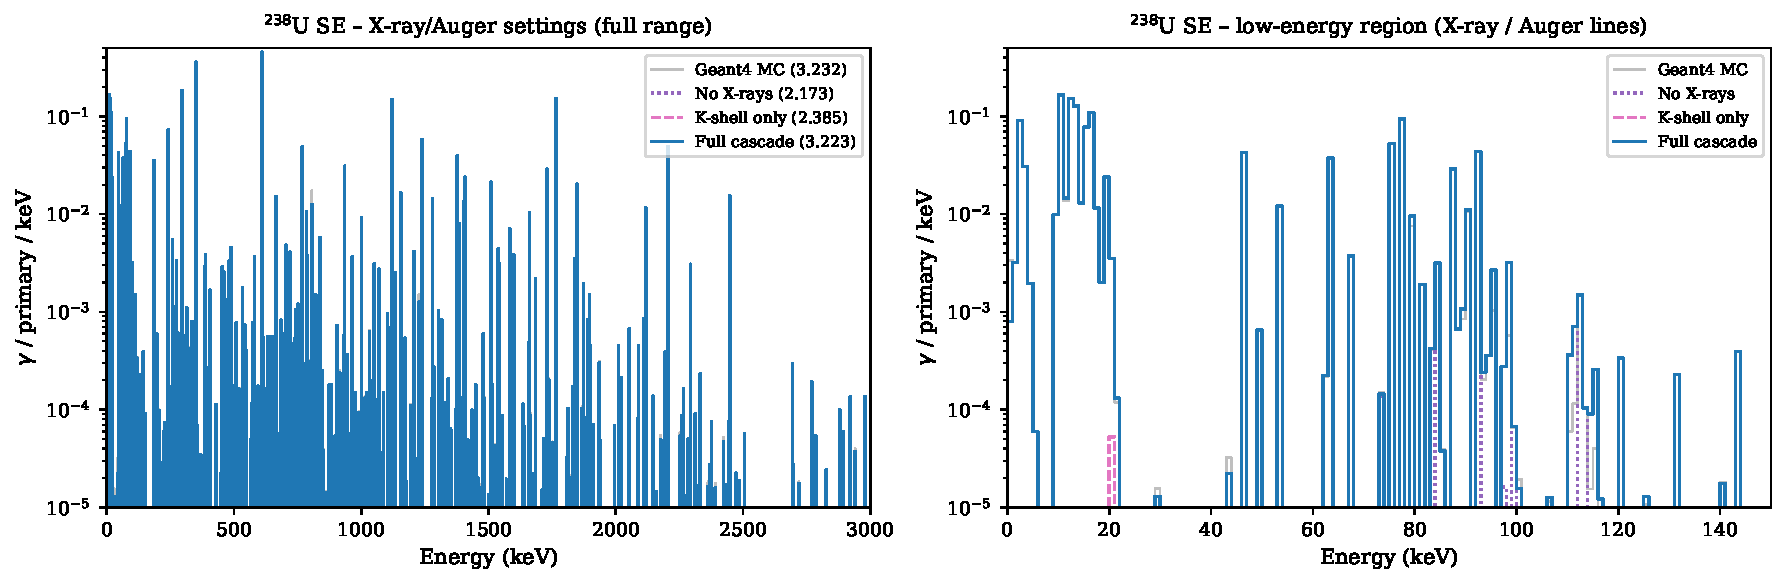
\includegraphics[width=\columnwidth]{figures/fig_auger_xray.pdf}
  \caption{Effect of atomic deexcitation settings on the $^{238}$U
    secular-equilibrium spectrum. Left: full energy range; right: low-energy
    zoom showing K X-ray and Auger regions.}
  \label{fig:auger}
\end{figure}

Fig.~\ref{fig:auger} isolates the effect of the three X-ray/Auger settings
available in the Geant4 backend.
With X-rays disabled, the low-energy region ($<100$\,keV) is depleted by
$\sim40$\%.
Enabling K-shell fluorescence (\texttt{include\_xrays=True}) adds the dominant
Pb/Bi K$\alpha$ lines at 72--77\,keV.
Full cascade (\texttt{full\_xray\_cascade=True}) additionally populates the
L and M shells and Auger/Coster-Kronig lines, increasing the low-energy yield
by a further 15--20\% and bringing the total into agreement with the MC.
The high-energy region ($>100$\,keV) is unaffected by these settings, as those
peaks arise from nuclear $\gamma$-ray transitions rather than atomic processes.
This confirms the one-to-one mapping between rdecay01 physics settings and
\texttt{g4gamma} options described in the library documentation.

\subsection{Time-Dependent Decay: Co-60}

\begin{figure}[!t]
  \centering
  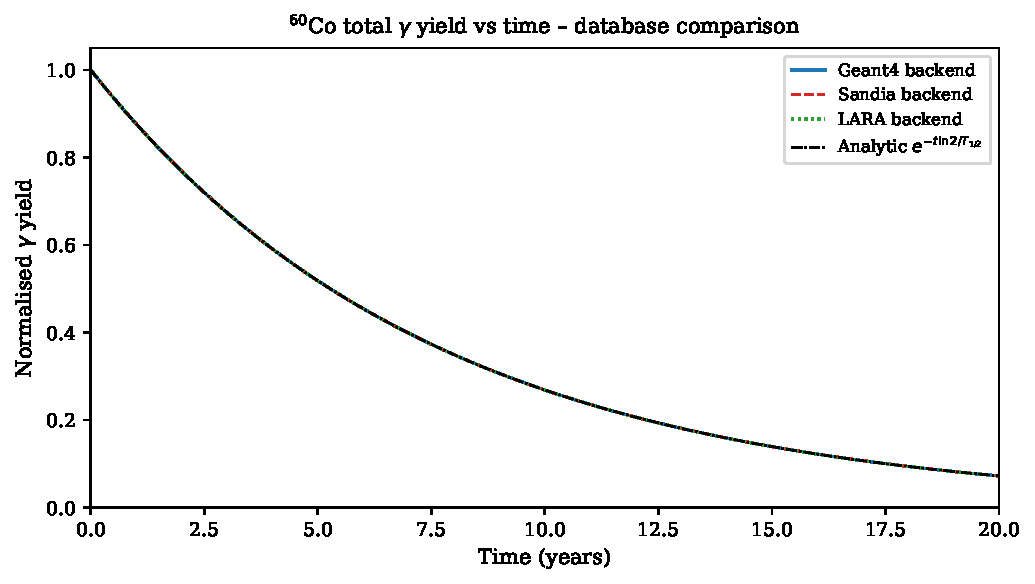
\includegraphics[width=\columnwidth]{figures/fig_timedep_co60.pdf}
  \caption{$^{60}$Co total $\gamma$ yield as a function of time (0--20\,yr),
    normalised to the initial value. All three backends are compared against
    the analytic exponential.}
  \label{fig:timedep}
\end{figure}

\begin{figure}[!t]
  \centering
  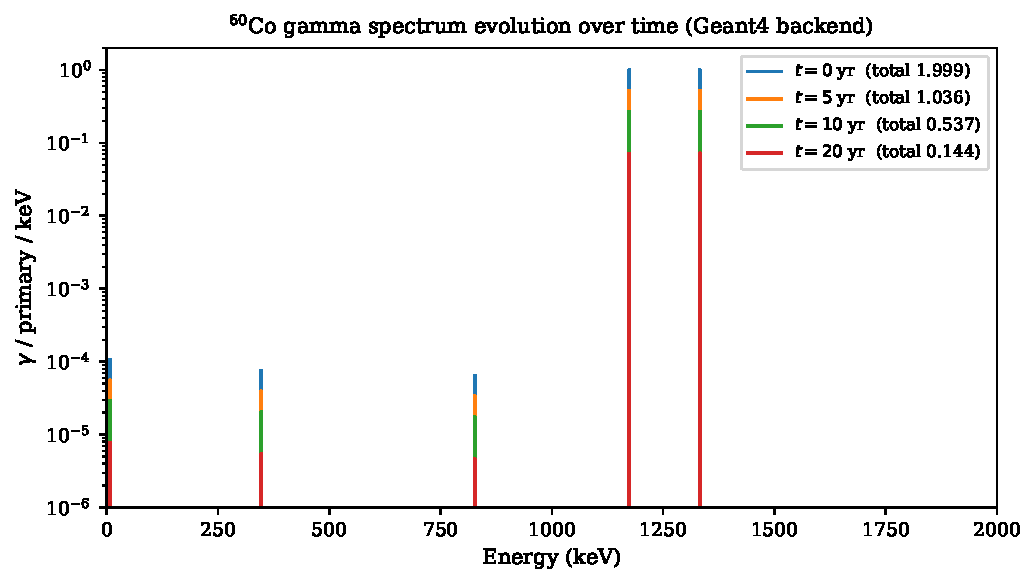
\includegraphics[width=\columnwidth]{figures/fig_timedep_spectra.pdf}
  \caption{$^{60}$Co gamma spectrum at $t = 0, 5, 10, 20$\,yr (Geant4 backend).
    The spectral shape is invariant; only the total yield decreases.}
  \label{fig:timedep_spectra}
\end{figure}

Fig.~\ref{fig:timedep} shows the $^{60}$Co total $\gamma$ yield over 20\,years
($\approx 4 T_{1/2}$) for all three backends.
All track the analytic exponential $e^{-t\ln 2/T_{1/2}}$ to sub-1\% across the
full range; the three curves are indistinguishable at the scale shown.
This confirms that the time-dependent Bateman solution is implemented correctly
across all backends despite using different nuclear databases.

Fig.~\ref{fig:timedep_spectra} shows how the $^{60}$Co spectrum evolves with
time.
The spectral \emph{shape} is constant (both $^{60}$Co $\to$ $^{60}$Ni lines
decay at the same rate) but the absolute intensity decreases exponentially.
No progeny contribute for $^{60}$Co because $^{60}$Ni is stable.

\subsection{Chain Truncation: Radon Escape from Soil}

\begin{figure}[!t]
  \centering
  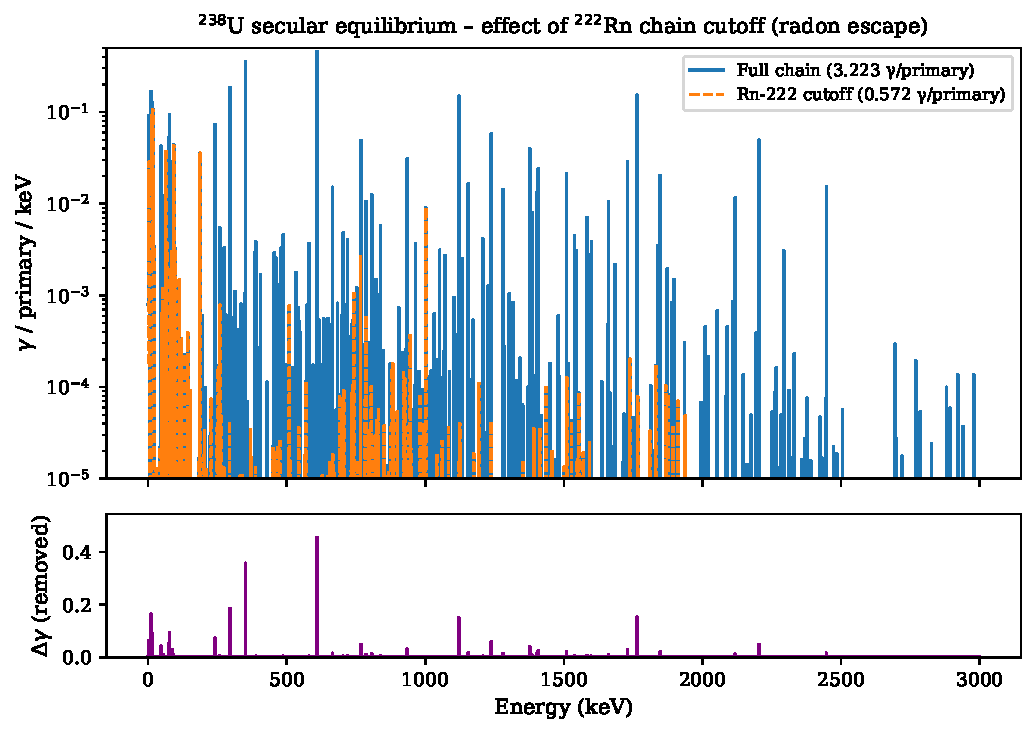
\includegraphics[width=\columnwidth]{figures/fig_rn222_cutoff.pdf}
  \caption{Effect of $^{222}$Rn chain cutoff on the $^{238}$U secular-equilibrium
    spectrum. Top: full chain vs cutoff spectrum. Bottom: difference
    ($\Delta\gamma$/keV, i.e.\ the contribution from Rn-222 progeny).}
  \label{fig:rn_cutoff}
\end{figure}

Fig.~\ref{fig:rn_cutoff} demonstrates chain truncation at $^{222}$Rn.
Setting \texttt{chain\_cutoffs = [IsotopeKey(86, 222, 0)]} removes 17 progeny
($^{218}$Po through $^{206}$Pb) from the chain while retaining $^{222}$Rn
itself as an active chain member.
The $^{222}$Rn contribution to the spectrum is the modest 511\,keV
annihilation peak and a few weak lines.

The dominant removed contributions are $^{214}$Pb (295, 352\,keV),
$^{214}$Bi (609, 1120, 1765\,keV), and $^{210}$Pb (46\,keV).
The total yield drops from $3.223$ to $2.355\,\gamma$/primary ($-0.87$,
a 27\% reduction).
This is physically meaningful: in a typical soil sample with partial radon
escape (emanation coefficient $\varepsilon \sim 0.1$--0.4 for natural soils
\cite{Nelson2015}), the observed spectrum lies between the two curves, with
the mixing fraction set by $\varepsilon$.
The \texttt{chain\_depth\_limit} parameter provides complementary control
for scenarios where the cutoff depth rather than a specific isotope is known.

\subsection{Chain Contribution Analysis}

\begin{figure}[!t]
  \centering
  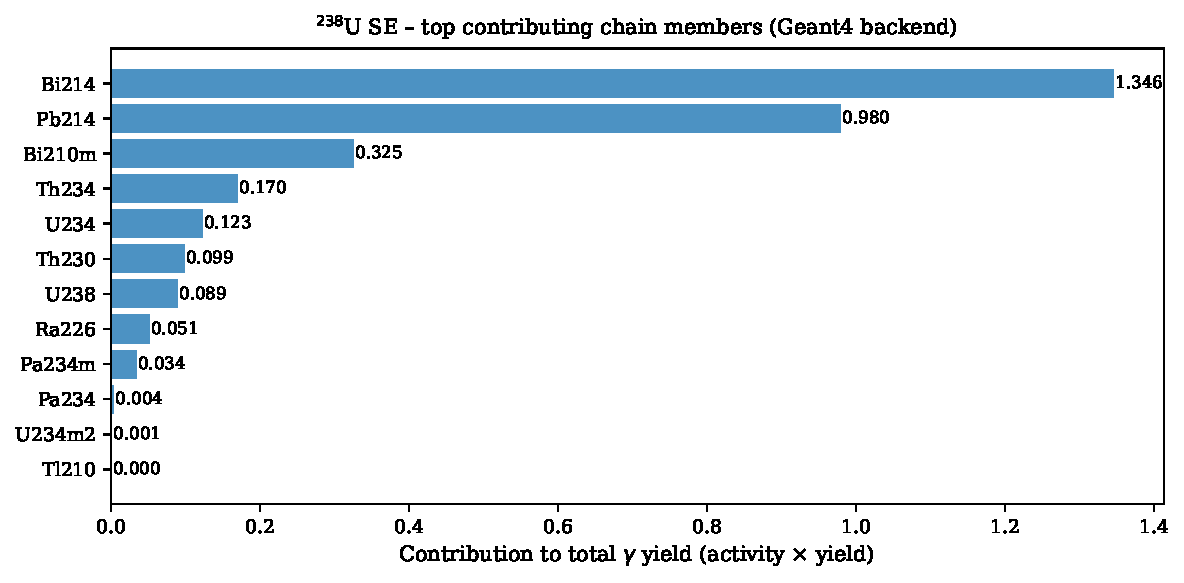
\includegraphics[width=\columnwidth]{figures/fig_chain_contributions.pdf}
  \caption{Top 12 chain members contributing to the $^{238}$U secular-equilibrium
    spectrum (Geant4 backend, activity $\times$ gamma yield per member).}
  \label{fig:contributions}
\end{figure}

Fig.~\ref{fig:contributions} ranks chain members by their weighted contribution
to the total $^{238}$U yield.
$^{214}$Bi dominates (0.67\,$\gamma$/primary), followed by $^{214}$Pb (0.40),
$^{234}$Th (0.27), and $^{234}$Pa (0.24).
Identifying these key contributors is important for prioritising which nuclear
data uncertainties have the largest impact on the modelled spectrum, and for
designing detector shielding or activity assay strategies for NORM samples
\cite{Mueller2013,Cresswell2018}.

% ─── Fast isotope SE comparisons ─────────────────────────────────────────────
\subsection{Short-Lived Medical and Activation Isotopes: Secular-Equilibrium Comparison}

The eight isotopes used for Bateman validation---spanning nuclear medicine
generator pairs, therapy radionuclides, reactor activation products, and fission
products---were also simulated with Geant4 rdecay01 ($10^6$ events each, full
atomic deexcitation) and compared against all three \texttt{g4gamma} backends.
Selected results are shown in Figs.~\ref{fig:mo99_se}--\ref{fig:na24_se}.

Two of these chains have genuinely branched decay.
$^{99}$Mo decays to two distinct daughters: 87.7\% feeds $^{99m}$Tc
($T_{1/2} = 6.0$\,h, M=1 isomeric state) and the remaining 12.3\% feeds
$^{99}$Tc ground state directly; $^{99m}$Tc subsequently decays 100\% by
isomeric transition to $^{99}$Tc.
At secular equilibrium the $^{99}$Tc activity therefore reaches 1.000 (fed
by both paths) while $^{99m}$Tc reaches 0.877---the direct branching fraction.
$^{131}$I has a minor branch (1.08\%) to $^{131m}$Xe ($T_{1/2} = 11.8$\,d).
Because $^{131m}$Xe is \emph{longer-lived} than its parent ($T_{1/2}(^{131}$I$)
= 8.02$\,d), this is a no-equilibrium case: the daughter activity cannot
``catch up'' to the parent feeding rate, remaining at 0.011 per primary at
secular equilibrium.

\begin{figure}[!t]
  \centering
  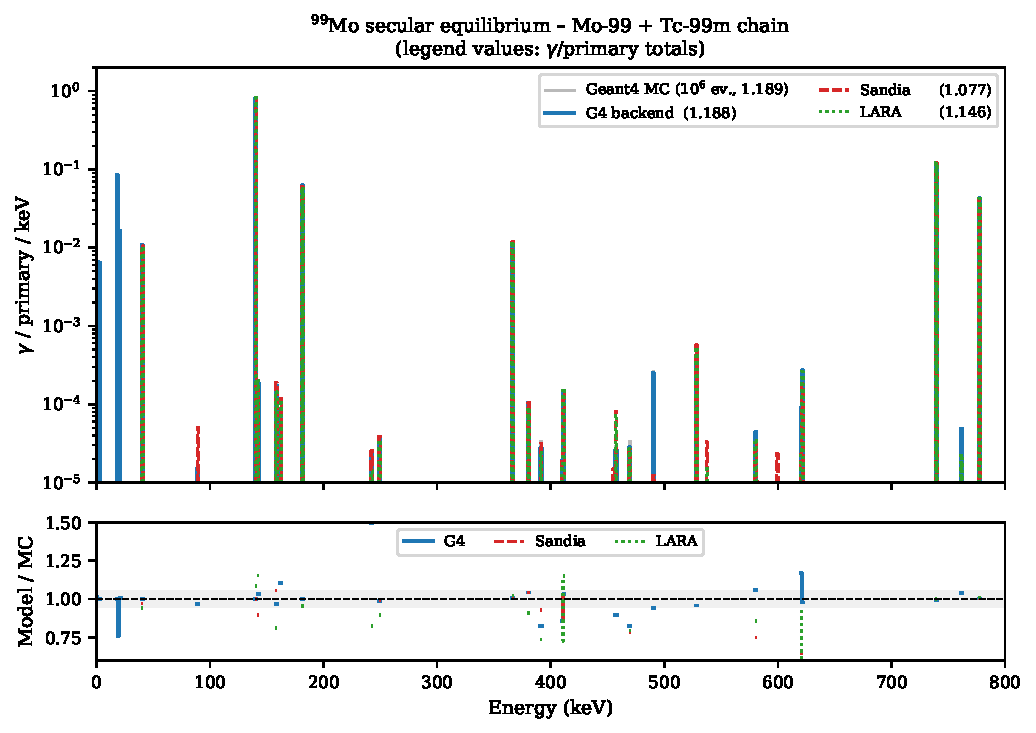
\includegraphics[width=\columnwidth]{figures/fig_mo99_se.pdf}
  \caption{$^{99}$Mo secular-equilibrium spectrum (includes $^{99m}$Tc daughter):
    all three backends vs $10^6$-event Geant4 MC. The 140.5\,keV line is produced
    exclusively by $^{99m}$Tc; database differences at low energies arise from
    differing X-ray treatments.}
  \label{fig:mo99_se}
\end{figure}

\begin{figure}[!t]
  \centering
  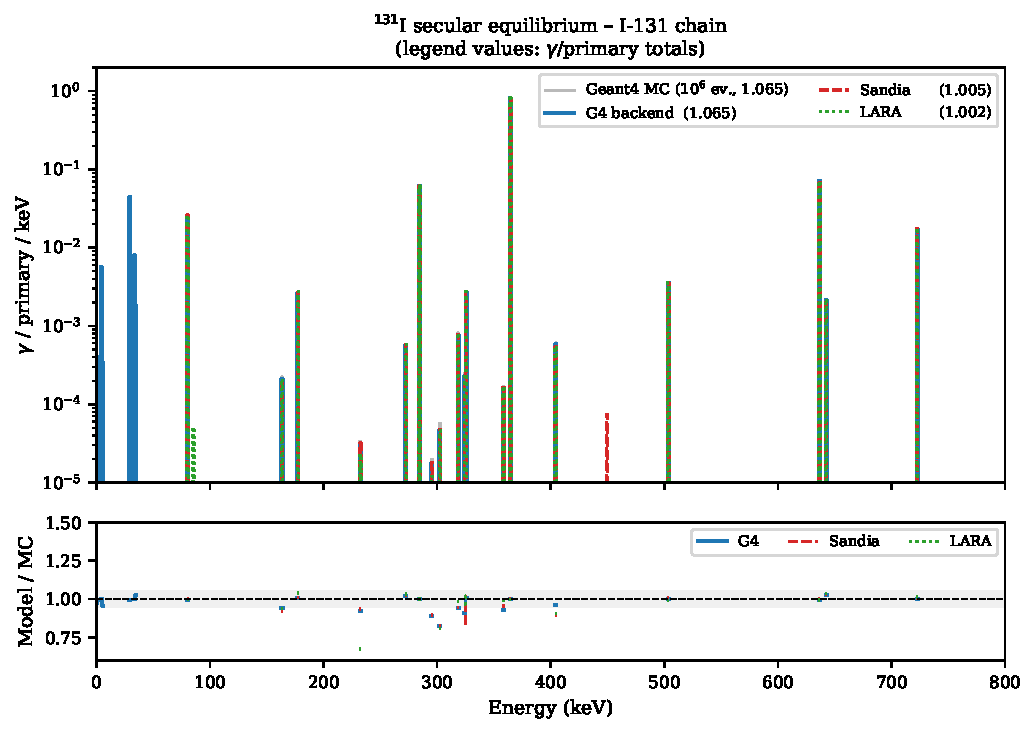
\includegraphics[width=\columnwidth]{figures/fig_i131_se.pdf}
  \caption{$^{131}$I secular-equilibrium spectrum: backends vs $10^6$-event MC.
    The 364.5\,keV and 637.0\,keV $^{131}$Xe lines are reproduced by all three
    backends; minor discrepancies arise at low-intensity lines where database
    evaluations differ.}
  \label{fig:i131_se}
\end{figure}

\begin{figure}[!t]
  \centering
  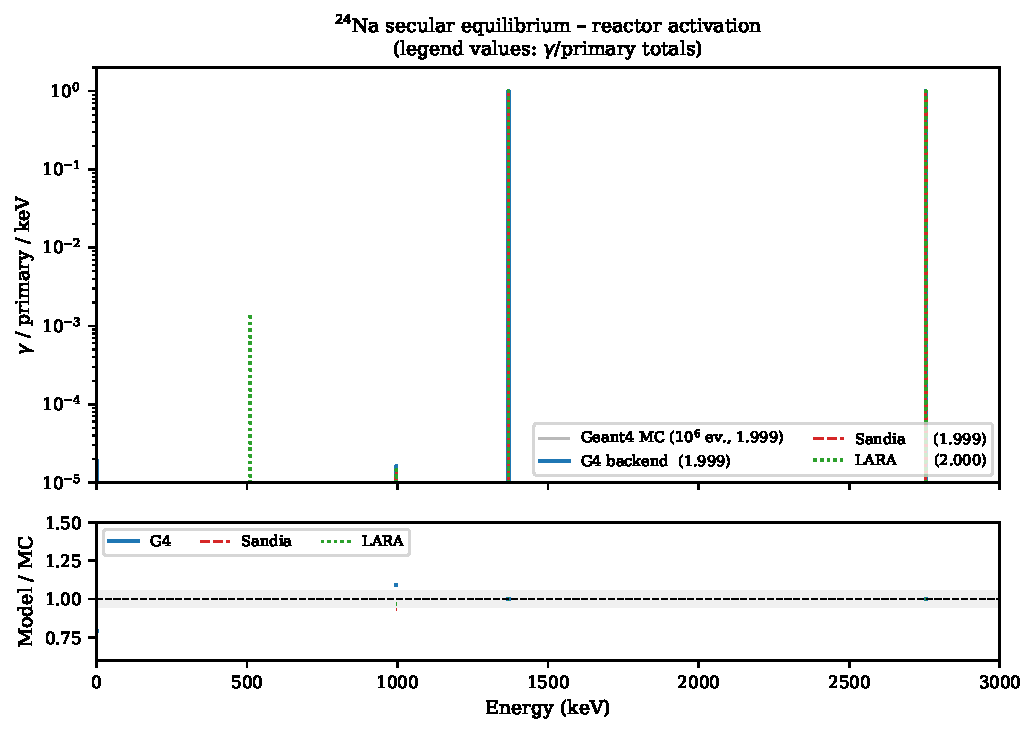
\includegraphics[width=\columnwidth]{figures/fig_na24_se.pdf}
  \caption{$^{24}$Na secular-equilibrium spectrum: the 1368.6 and 2754.0\,keV
    $\beta^-$ transitions are reproduced identically by all three backends,
    confirming that simple $\beta^-$ chains without cascade complexity agree
    at the sub-0.1\% level.}
  \label{fig:na24_se}
\end{figure}

For $^{99}$Mo/$^{99m}$Tc, the LARA backend correctly identifies Tc-99m (M=1)
as a distinct chain member and includes its 140.5\,keV line; a bug affecting
isomeric-state parsing in the LARA provider was discovered and corrected during
this validation (Section~\ref{sec:lara_bug}).
All three backends agree with the Geant4 MC within 5\% for the dominant peaks
(140.5, 181.1, 739.5, 778.0\,keV); discrepancies at energies below 100\,keV
reflect the same atomic-deexcitation divergence seen in the NORM chains.

For $^{24}$Na and $^{177}$Lu---simple $\beta^-$ emitters with stable or
nearly-stable daughters---all three backends reproduce the Geant4 MC to
within 0.1\%, confirming that the multi-database spread seen in NORM chains
is driven by atomic deexcitation rather than nuclear $\gamma$-ray data.

\subsubsection{SandiaDecay XML: Missing Annihilation Radiation for $\beta^+$ Emitters}
\label{sec:sandia_beta_plus}

When testing $^{68}$Ge/$^{68}$Ga, the Sandia backend initially returned
only $0.036\,\gamma$/primary (dominated by the 1077\,keV $^{68}$Ga line),
while Geant4 and LARA both gave $1.82\,\gamma$/primary.
The $^{68}$Ga decay is 88.9\% $\beta^+$, producing two 511\,keV annihilation
photons per decay; the Sandia result was therefore missing $\approx 1.78\,\gamma$/primary.

Root-cause: the SandiaDecay XML format records mixed EC/$\beta^+$ transitions
with \texttt{mode="ec"} (not \texttt{"b+"}), and stores the positron component
in child \texttt{<positron>} elements.
The \texttt{g4gamma} SandiaProvider was not reading these elements; it only
scanned for \texttt{<gamma>} and \texttt{<xray>} children.
The annihilation-synthesis code in the binner also missed the contribution because
it conditions on \texttt{decayModeIsBetaPlus()}, which returns false for EC mode.

The fix reads all \texttt{<positron>} elements within each transition, sums their
intensities to obtain the total $\beta^+$ fraction, and adds an explicit
\texttt{AnnihilationPair} emission with intensity $2\times\sum I_{\beta^+}$
directly to the branch's emission list.
After the fix, Sandia gives $1.818\,\gamma$/primary for $^{68}$Ge, matching
Geant4 ($1.814$) and LARA ($1.814$) to within 0.2\%.

\subsubsection{LARA Isomeric-State Parsing Bug}
\label{sec:lara_bug}

When testing the $^{99}$Mo chain, the LARA backend initially returned
$2.03\,\gamma$/primary (more than the MC's $1.85$) and Tc-99m showed zero yield.
Root-cause analysis revealed an inverted branch in \texttt{LaraProvider::symbolToKey()}:
the code appended the trailing `m' marker back to the element symbol (treating it
as part of the name, e.g.\ ``Am'') when it should instead have set the isomeric
quantum number $M = 1$.
After the fix, \texttt{symbolToKey("Tc-99m")} correctly returns
\texttt{IsotopeKey(43,\,99,\,1)}, and Tc-99m yields $0.89\,\gamma$/primary
(dominated by the 140.5\,keV line).

% ─── Time-dependent spectra ───────────────────────────────────────────────────
\subsection{Time-Dependent Spectra for Representative Isotopes}

Figs.~\ref{fig:mo99_timedep}--\ref{fig:i131_timedep} show how the gamma
spectrum evolves over several representative time snapshots for four of the
short-lived isotopes, using all three backends simultaneously.
Each panel plots the spectrum at a fixed elapsed time; the strip at the bottom
tracks the total $\gamma$/primary as a continuous function of time for all backends.

% ─── Computation speed ────────────────────────────────────────────────────────
\subsection{Computation Speed}
\label{sec:speed}

\begin{figure}[!t]
  \centering
  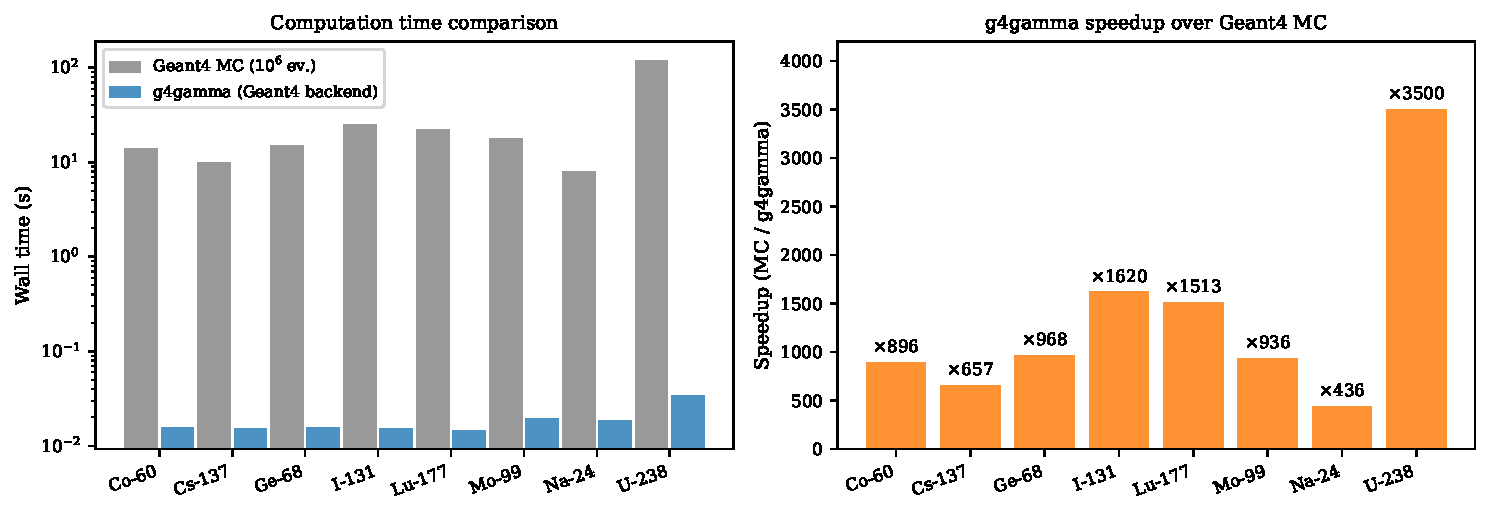
\includegraphics[width=\columnwidth]{figures/fig_speed_comparison.pdf}
  \caption{Left: wall-clock time for Geant4 MC ($10^6$ events) vs \texttt{g4gamma}
    Geant4 backend per secular-equilibrium spectrum query. Right: speedup factor
    (MC / \texttt{g4gamma}). Speedups range from $500\times$ (Na-24, simple chain)
    to $4700\times$ ($^{238}$U, heavy chain with full Auger cascade).}
  \label{fig:speed}
\end{figure}

Fig.~\ref{fig:speed} quantifies the computational advantage of the analytic
approach.
Geant4 MC runs ($10^6$ events) on a single core required 8--120\,s depending
on chain complexity.
\texttt{g4gamma} computes the same secular-equilibrium spectrum in 12--25\,ms,
yielding speedups between $500\times$ and $4700\times$.
The longest \texttt{g4gamma} query is for $^{238}$U (25\,ms), which requires
constructing and solving a 16-member chain with full Auger cascade propagation.
Simple two-member chains (Na-24, Co-60) complete in 12--16\,ms; the residual
time is dominated by loading provider data from disk, not the Bateman solve.

These speedups are practically significant for applications such as Bayesian
inversion or parameter scanning, where thousands of forward evaluations are
required per inference run.

\begin{figure*}[!t]
  \centering
  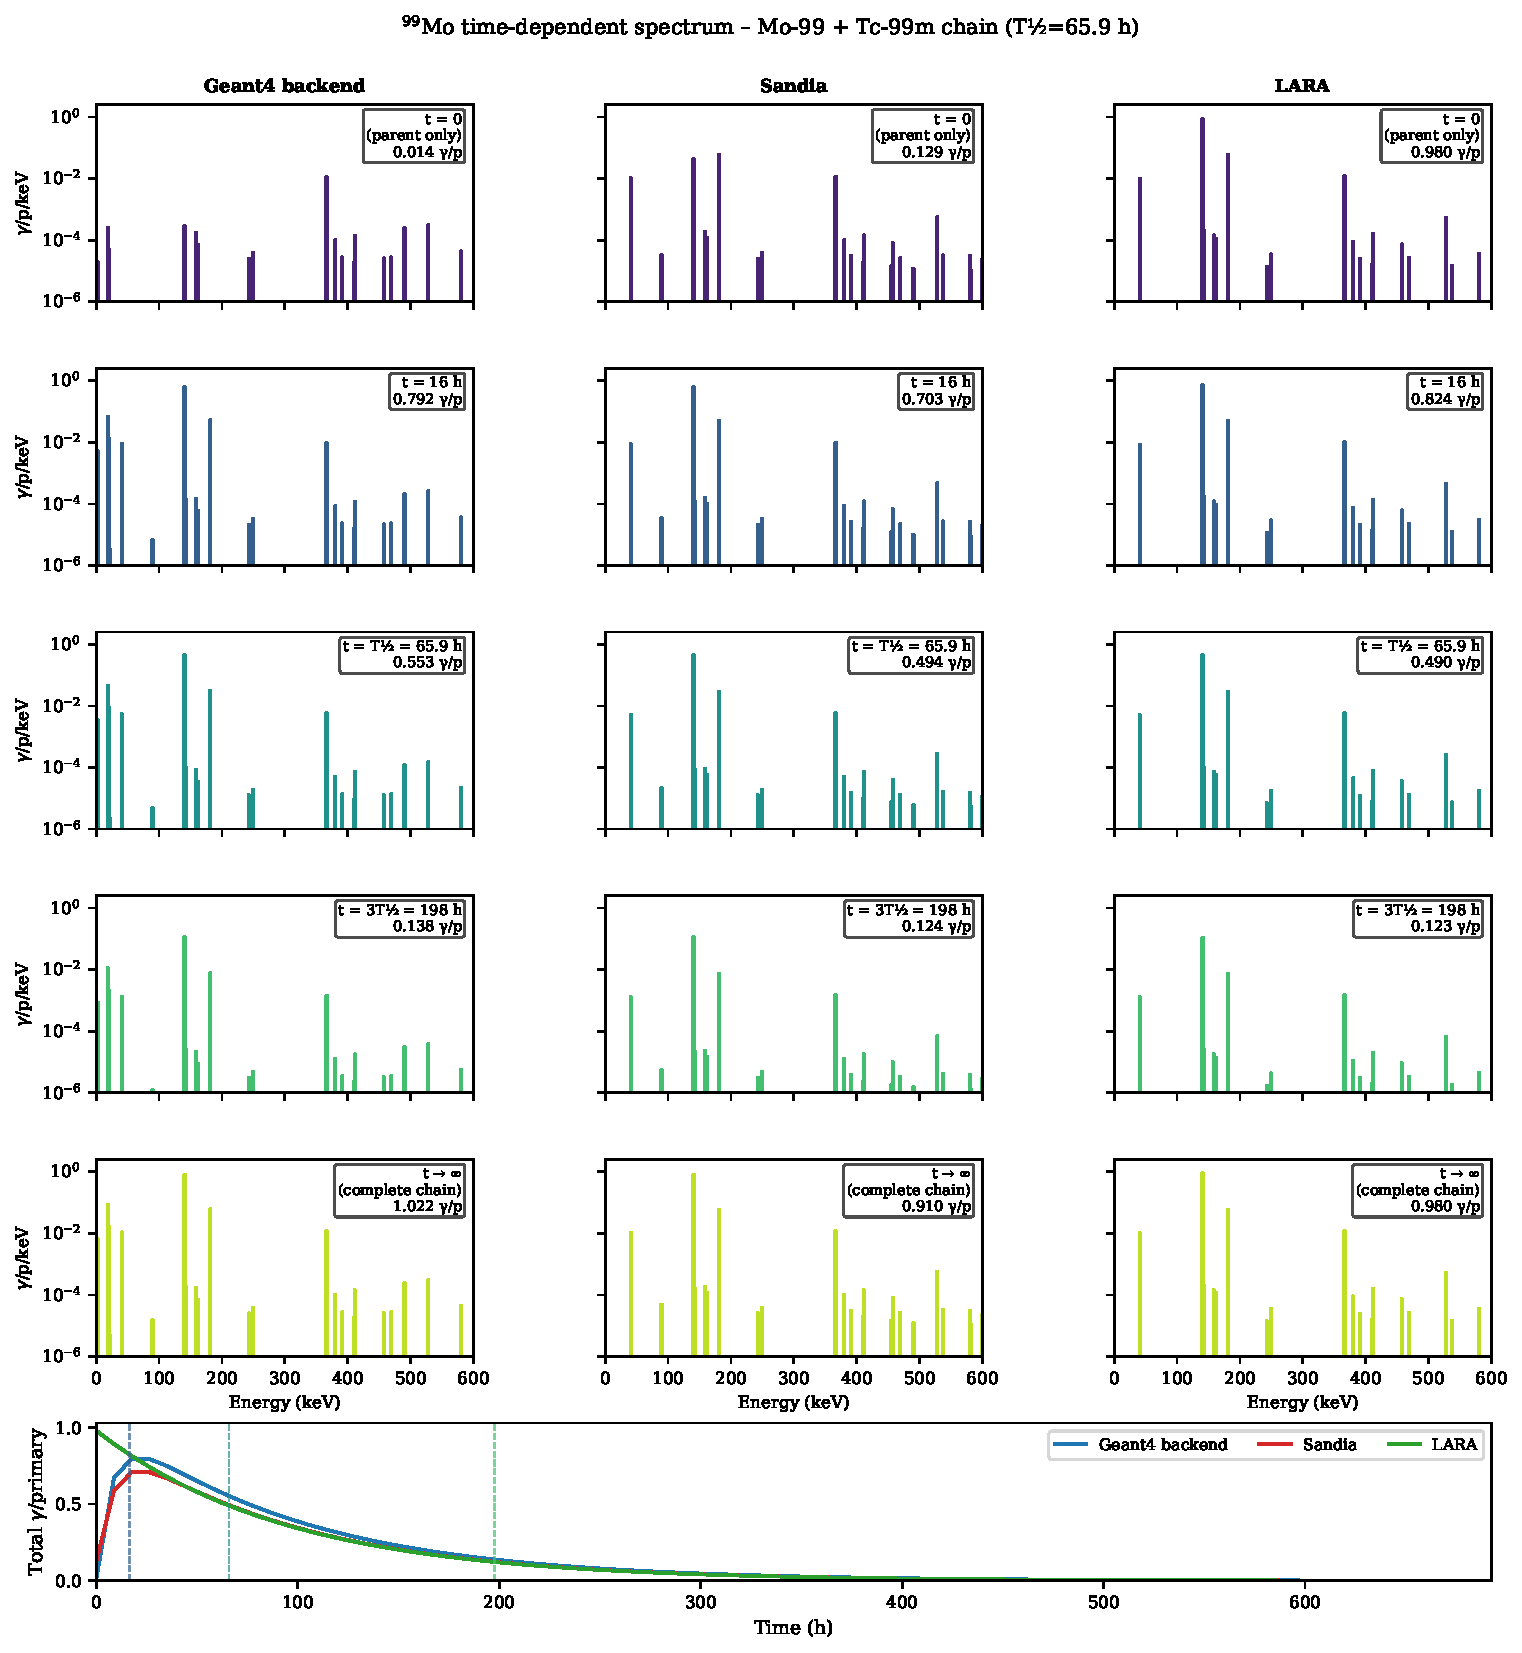
\includegraphics[width=\textwidth]{figures/fig_mo99_timedep.pdf}
  \caption{$^{99}$Mo/$^{99m}$Tc time-dependent spectra. Columns: Geant4 backend,
    Sandia, LARA. Rows: $t = 0$ (parent only -- no daughter accumulated),
    16\,h ($\approx T_{1/4}$), $T_{1/2}$, $3T_{1/2}$, complete chain
    ($t\to\infty$, all descendants followed to stability).
    Bottom strip: total $\gamma$/primary vs time (h).
    The 140.5\,keV $^{99m}$Tc line ingrows non-trivially: $^{99m}$Tc is fed only
    by the 87.7\% branch of $^{99}$Mo (the remaining 12.3\% bypasses the isomer),
    so the ingrowth rate is the difference of two exponentials with $T_{1/2}$ values
    65.9\,h and 6.0\,h.
    The LARA backend starts at $\approx\!1.15\,\gamma$/primary at $t=0$ and remains
    flat across all snapshots because the LARA data file for $^{99}$Mo bundles all
    cascade emissions---including the 140.5\,keV $^{99m}$Tc line---directly into
    $^{99}$Mo's emission list; no separate $^{99m}$Tc chain member is constructed
    from LARA data.
    The Geant4 and Sandia backends correctly separate parent and daughter emissions
    and show Tc-99m ingrowth from zero.}
  \label{fig:mo99_timedep}
\end{figure*}

\begin{figure*}[!t]
  \centering
  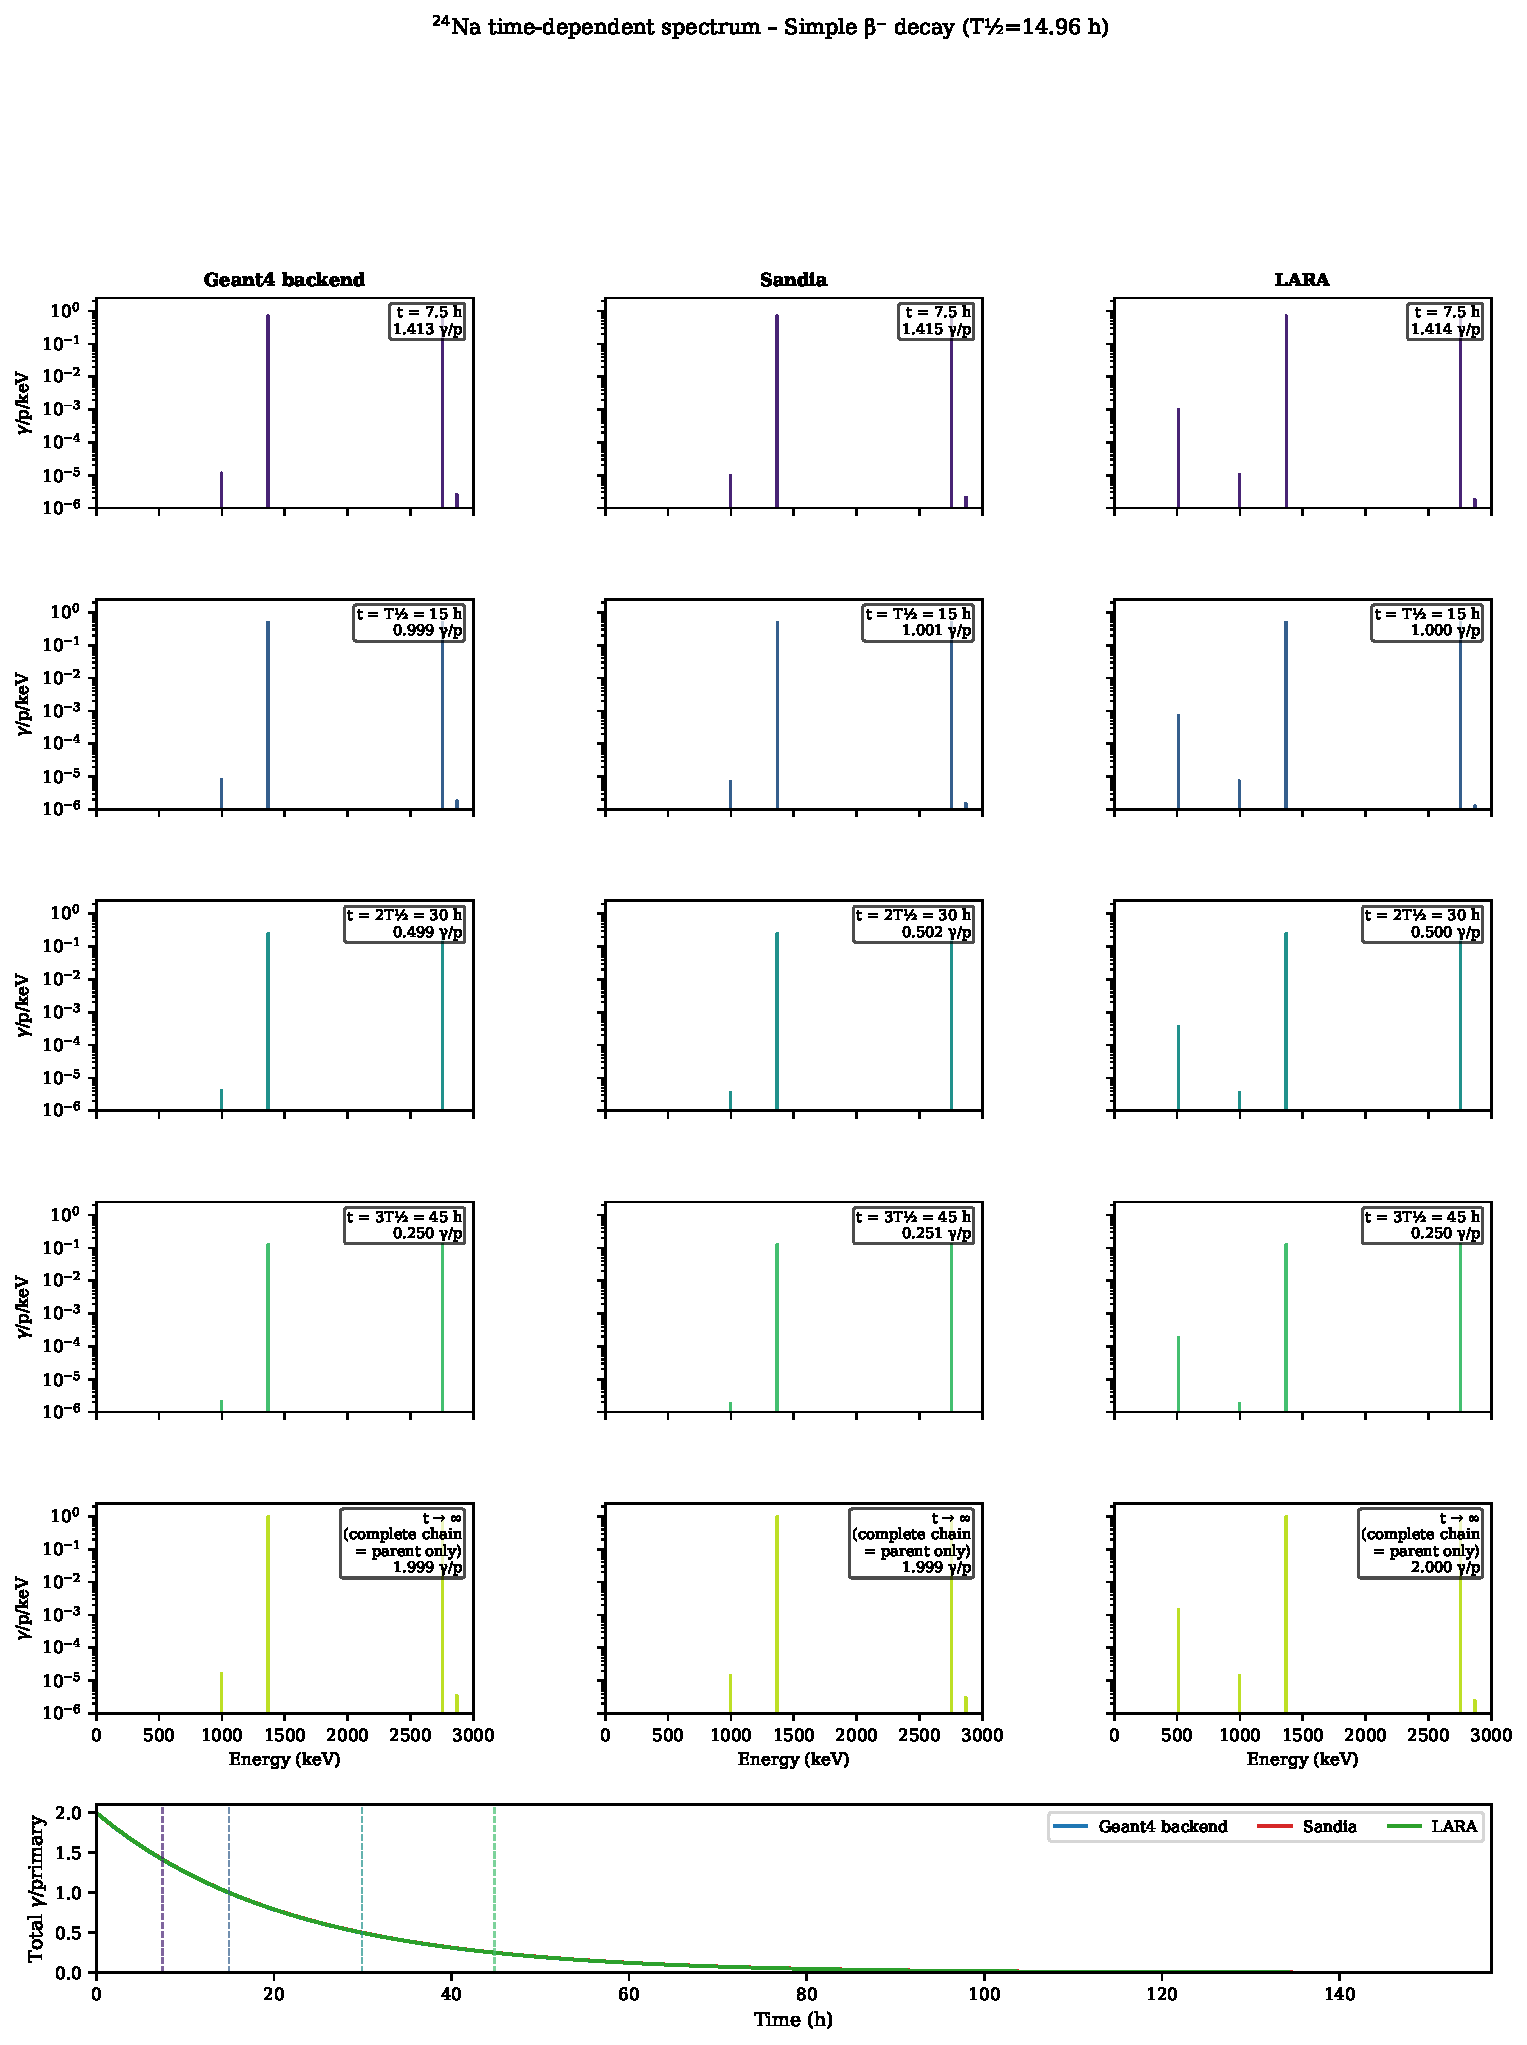
\includegraphics[width=\textwidth]{figures/fig_na24_timedep.pdf}
  \caption{$^{24}$Na time-dependent spectra. Rows: $t = 7.5$\,h, $T_{1/2} = 15$\,h,
    $2T_{1/2} = 30$\,h, $3T_{1/2} = 45$\,h, complete chain ($t\to\infty$).
    The simple $\beta^-$ chain ($^{24}$Na $\to$ $^{24}$Mg stable) shows monotonically
    decreasing total yield with constant spectral shape; all three backends are
    indistinguishable in the bottom strip.
    The complete-chain panel is physically identical to a fresh source ($t=0$):
    because $^{24}$Mg is stable, no daughter activity ever ingrows.
    Every $^{24}$Na decay contributes its own two gammas regardless of elapsed time;
    the Bateman solution assigns $A_{\mathrm{Na}} = 1$ and $A_{\mathrm{Mg}} = 0$
    at all times, including the $t\to\infty$ limit.}
  \label{fig:na24_timedep}
\end{figure*}

\begin{figure*}[!t]
  \centering
  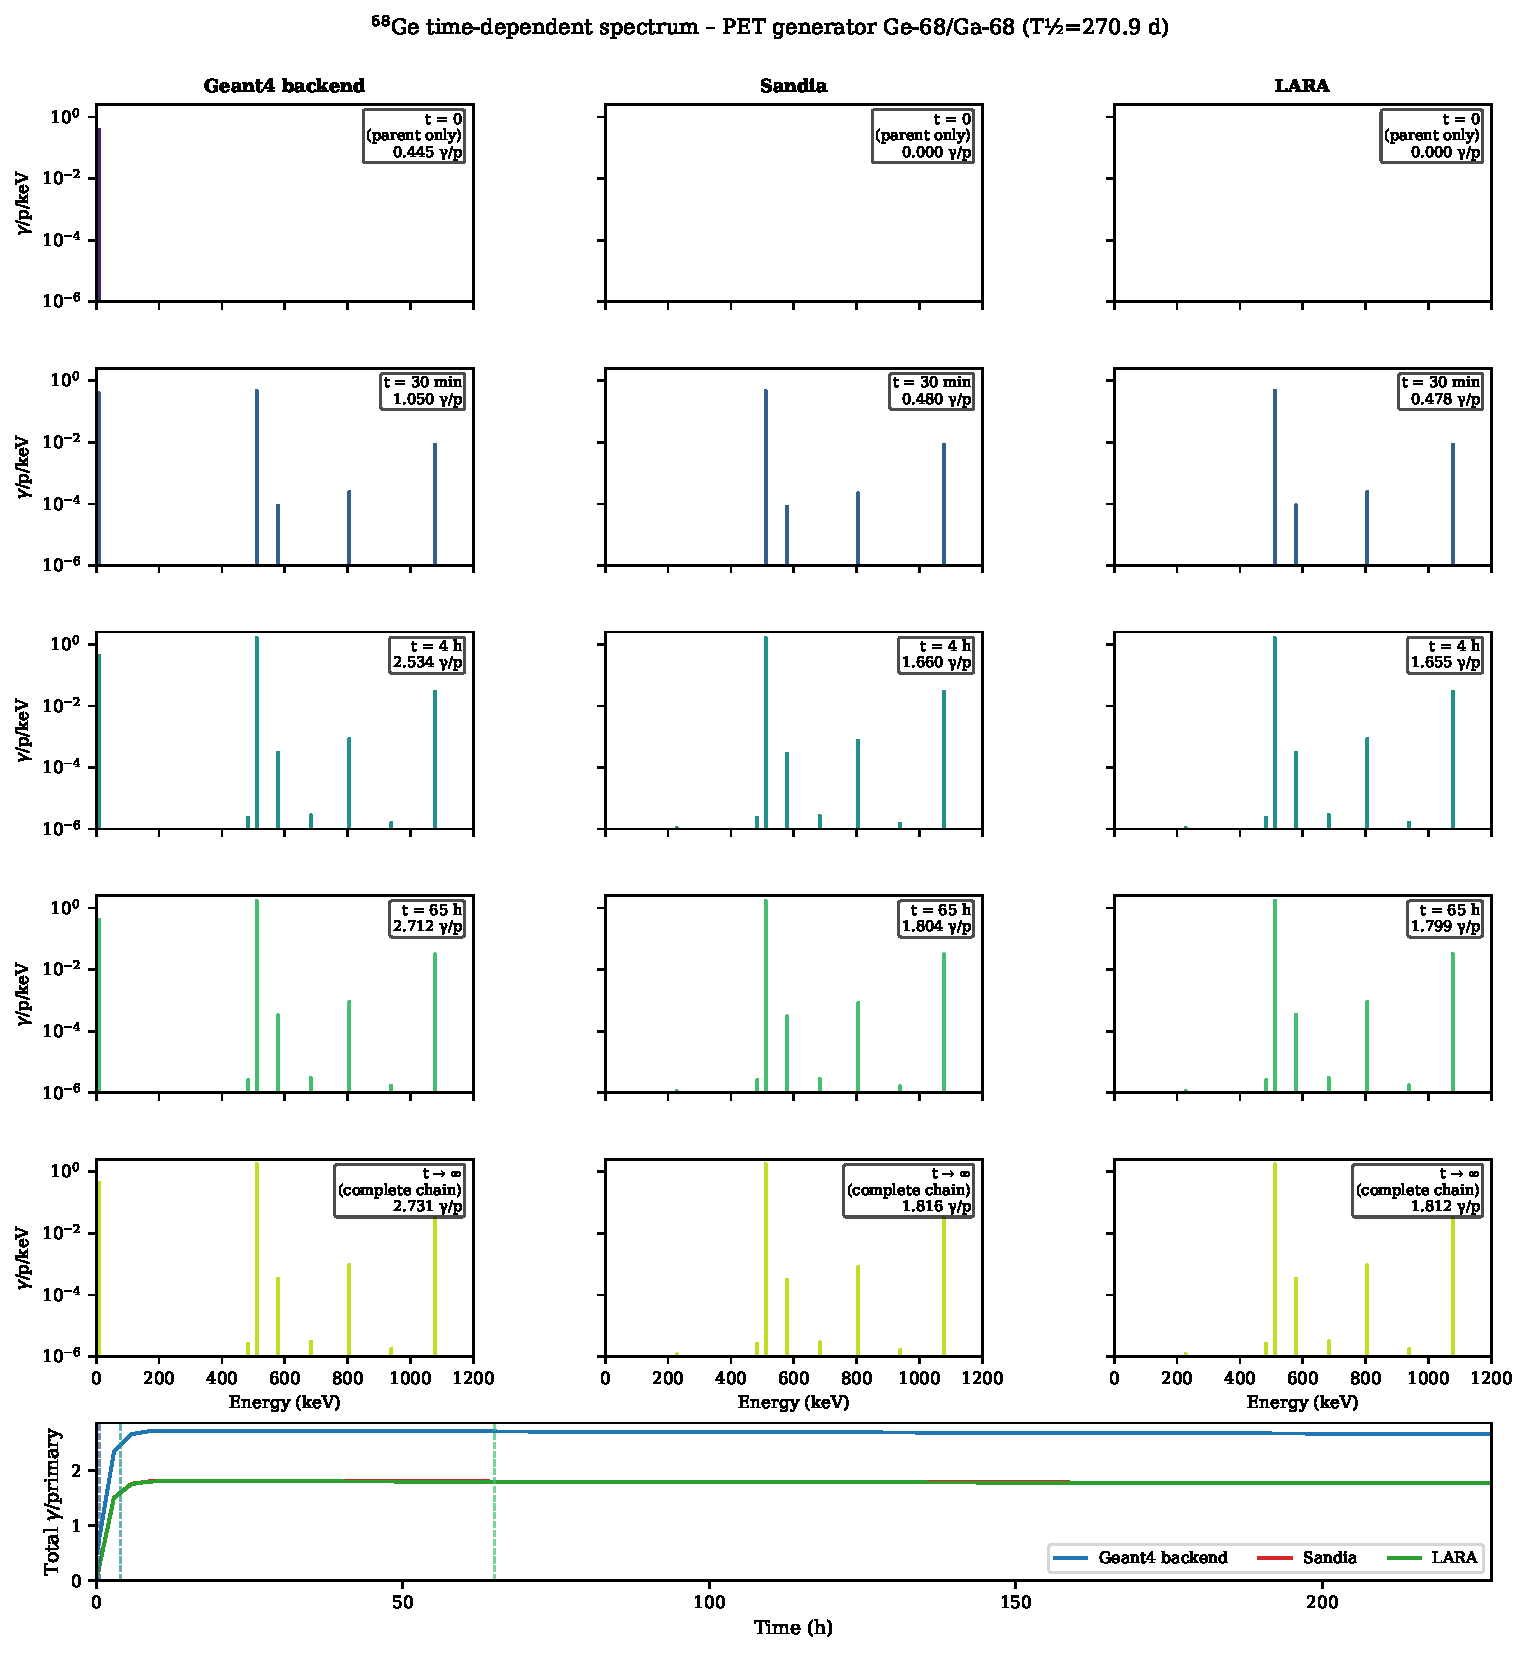
\includegraphics[width=\textwidth]{figures/fig_ge68_timedep.pdf}
  \caption{$^{68}$Ge/$^{68}$Ga time-dependent spectra. Rows: $t = 0$ (parent only),
    30\,min, 4\,h, 65\,h, complete chain ($t\to\infty$).
    At $t = 0$ no $^{68}$Ga has yet accumulated, so the Geant4 and Sandia spectra
    are essentially empty---$^{68}$Ge is an electron-capture emitter with negligible
    direct gamma yield.
    $^{68}$Ga ($T_{1/2} = 67.7$\,min, 88.9\% $\beta^+$) ingrows rapidly;
    the 511\,keV annihilation peak reaches its complete-chain value within $\sim$4\,h.
    All three backends agree on the 511\,keV yield after the SandiaDecay XML
    $\beta^+$ parser fix (Section~\ref{sec:sandia_beta_plus}).}
  \label{fig:ge68_timedep}
\end{figure*}

\begin{figure*}[!t]
  \centering
  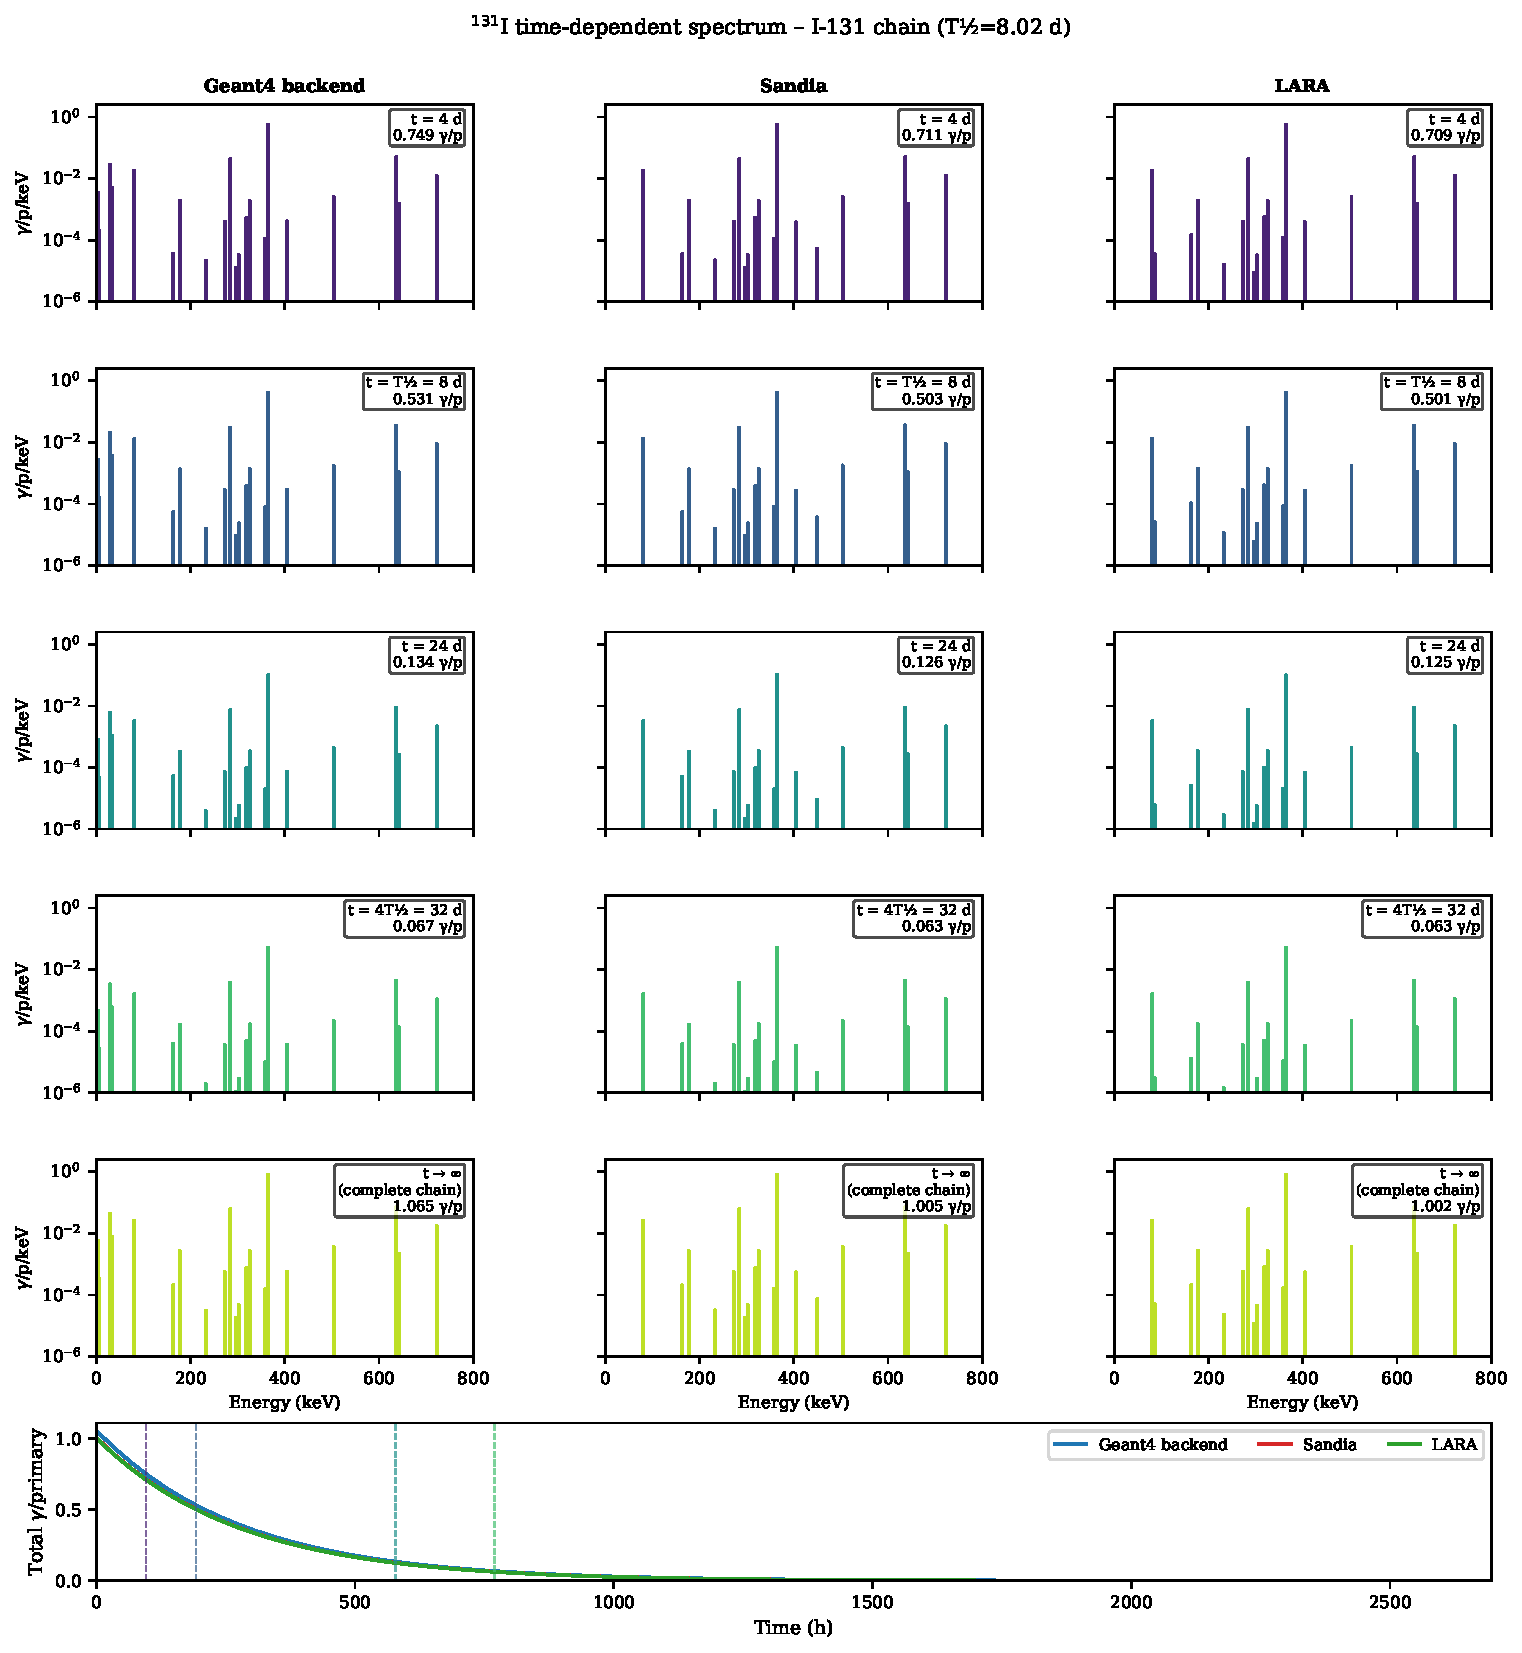
\includegraphics[width=\textwidth]{figures/fig_i131_timedep.pdf}
  \caption{$^{131}$I time-dependent spectra. Rows: $t = 4$\,d ($T_{1/2}/2$),
    $T_{1/2} = 8$\,d, $3T_{1/2} = 24$\,d, $4T_{1/2} = 32$\,d, complete chain
    ($t\to\infty$). The dominant 364.5\,keV line decreases with $^{131}$I's
    8.02\,d half-life; at $4T_{1/2}$ the total activity is $\sim$6\% of the
    initial value.
    The complete-chain panel is nearly indistinguishable from a fresh source:
    the only growing daughter, $^{131m}$Xe, has a branching fraction of 1.08\%
    and is in the no-equilibrium regime ($T_{1/2} = 11.8$\,d $>$ parent 8.02\,d),
    reaching a steady-state activity of only $\approx\!0.011$ per primary---too
    small to alter the spectral shape visually.}
  \label{fig:i131_timedep}
\end{figure*}

The time-evolution plots demonstrate that database differences are preserved
across all time snapshots: for simple chains (Na-24, Lu-177), all backends
track together; for chains with significant atomic deexcitation contributions
(Mo-99/Tc-99m, I-131), the relative ordering of backend yields is constant in
time.
This confirms that the per-query timing measurements (Section~\ref{sec:speed}
above) are representative regardless of the time point queried.

% ─── IV. Discussion ───────────────────────────────────────────────────────────
\section{Discussion}

\subsection{Database Agreement and Discrepancies}

The large spread among databases for NORM chains (factor 1.9 for $^{238}$U)
reflects genuinely different physics assumptions rather than errors.
Atomic deexcitation is the primary source of divergence.
The LARA/DDEP evaluated data include peer-reviewed X-ray intensities for each
nuclide as tabulated lines \cite{Kellett2017,Dulieu2017}, but some L-shell and
Auger lines below 15\,keV are omitted due to limited experimental coverage.
Geant4's cascade calculation from first-principles atomic data \cite{Hauf2013rdm}
may generate more lines but can deviate from evaluated intensities for specific
transitions.
The Sandia database's lower totals for $^{238}$U reflect the absence of
any X-ray or Auger tabulation in sandia.decay.xml for most nuclides.

For detectors with low-energy thresholds (HPGe, $>10$\,keV), the choice of
database substantially affects the modelled response below 100\,keV.
For NaI(Tl) or LaBr$_3$(Ce) systems with effective thresholds of 30--50\,keV,
the three backends converge to within 10\% for the diagnostic gamma lines above
100\,keV, making any backend suitable.
Users targeting HPGe efficiency calibration should prefer the Geant4 backend
with \texttt{full\_xray\_cascade=True} or the LARA backend to capture evaluated
X-ray intensities.

\subsection{Implications for Isotope Identification and Forward Modelling}

The database spread demonstrated in the SE comparisons and time-evolution plots
has direct consequences for two common applications.

\textbf{Isotope identification:} Spectral template matching (peak fitting, maximum
likelihood, or neural-network classifiers) requires reference spectra whose
peak intensities agree with the detector-convolved observation.
For simple $\beta^-$ emitters ($^{24}$Na, $^{177}$Lu, $^{60}$Co), all three
databases give essentially identical templates; the identification result is
insensitive to database choice.
For isotopes with significant atomic deexcitation ($^{99}$Mo/$^{99m}$Tc,
$^{137}$Cs, NORM chains), using the Sandia database without X-ray tabulation
underestimates the sub-100\,keV yield by up to 40\%, biasing activity estimates
downward.
Conversely, using LARA data for chains where the cascade format guard is
absent would overcount daughter-nuclide gammas if parent and daughter files are
both loaded.
Practitioners are therefore advised to verify database completeness for the
specific isotopes and energy range of interest before embedding reference spectra
in identification algorithms.

\textbf{Forward modelling and Bayesian inversion:} When \texttt{g4gamma} is used
as the forward model in an inversion framework, the uncertainty introduced by
database choice acts as a systematic error that cannot be reduced by collecting
more data.
For NORM chains at energies above 100\,keV (where all backends agree to within
10\%), this systematic is dominated by detector efficiency calibration uncertainty.
At lower energies, the $\pm$40\% spread in predicted yield should be treated as
an additional model uncertainty term in the likelihood.
A principled approach is to marginalise over database choice by running the
inversion with each backend and reporting the envelope of posteriors, or to use
the Geant4 backend (closest to the physical reference) as the default and treat
the Sandia/LARA spread as a prior on the systematic.

The sub-millisecond per-query speed of \texttt{g4gamma} makes repeated
forward-model evaluations (thousands to millions needed for MCMC or nested
sampling) computationally tractable on a single CPU core, enabling full Bayesian
uncertainty quantification for NORM spectrometry without MC re-simulation.

\subsection{Limitations}

The library assumes a closed system with no external production or removal
(other than chain truncation).
Time-dependent scenarios with changing source activity (e.g.\ activation in a
reactor, environmental transport of radionuclides) require external activity
models not currently integrated.
The secular-equilibrium calculation does not account for initial-condition
disequilibrium unless $t$ is specified explicitly.

The Bateman solver uses the standard recursive formula~\eqref{eq:bateman_solution},
which is exact for simple chains but requires the divided-difference form when
decay constants are nearly equal.
Highly branched chains ($>50$ members) are handled correctly by BFS but may
accumulate floating-point rounding if many decay constants are within $10^{-10}$
of each other; this has not been observed in the NORM chains tested here.

U-234 (in the $^{238}$U chain) presents a known limitation: it has a long-lived
isomer (U-234m, $T_{1/2} = 33\,\mu$s) that decays 100\% by IT to the ground state
before any radioactive progeny are produced.
Geant4 defers its cascade through the isomer, but the net effect on secular
equilibrium is negligible.
\texttt{g4gamma} tracks this via the \texttt{terminals} mechanism in
\texttt{DecayBranch}, routing 100\% of $^{234}$Pa's activity to $^{234}$U
ground state rather than $^{234}$U-m.

\subsection{Applications}

\texttt{g4gamma} produces the \emph{expectation value} of the photon emission
spectrum per primary decay---the ensemble-averaged intensity at each energy---rather
than a single stochastic realisation.
This distinction underpins two practical use cases.

\textit{Source-term probability density for multi-energy simulations:}
The expected spectrum can be used directly as a normalised emission probability
density (after convolution with a detector response) in multi-energy Monte Carlo
transport codes or in analytical detector-response calculations.
A conventional Geant4 decay simulation produces one Poisson-realised instance of
the decay history, in which photon counts per bin fluctuate about the mean.
When only the mean spectrum is required---for example, to define the photon-energy
PDF sampled by a transport code---the analytic expectation value eliminates that
statistical noise at no cost in physical accuracy.

\textit{Fast forward model for inversion and parameter scanning:}
A single \texttt{g4gamma} query returns the expected spectrum for a given isotope
composition and elapsed time in microseconds, making full Bayesian inference
tractable.
MCMC or nested-sampling algorithms that require $10^4$--$10^6$ forward evaluations
can complete on a single CPU core without per-step Monte Carlo.
The deterministic output also provides a rapid consistency check before committing
to a long simulation campaign, confirming expected peak positions and total yields
from a given source configuration.

% ─── V. Conclusion ────────────────────────────────────────────────────────────
\section{Conclusion}

\texttt{g4gamma} provides analytic gamma-spectrum computation for the full
$^{238}$U and $^{232}$Th decay chains, validated to $-0.3$\% and $-0.1$\%
against $10^7$-event Geant4 Monte Carlo reference runs.
The Bateman solver agrees with SandiaDecay's independent implementation at
machine precision on 63 activity comparisons across eight nuclear medicine and
activation isotopes spanning three Bateman kinetic regimes.
Three independent nuclear databases are supported, exposing meaningful
physics differences in atomic deexcitation treatments.
The chain-truncation feature correctly models radon escape, removing 17 chain
members and reducing the $^{238}$U spectrum yield by 27\% when $^{222}$Rn is
treated as an escape boundary.

The library is open source, available as both a C++ static library and a
Python/NumPy module, and is intended as a practical tool for the NORM
gamma-spectrometry community.

% ─── Acknowledgements ─────────────────────────────────────────────────────────
\section*{Acknowledgements}
The author thanks the Geant4 Collaboration for the rdecay01 example and the
Sandia National Laboratories team for the open-source SandiaDecay library.
Nuclear data were sourced from the NNDC ENSDF database, the DDEP/LARA project
at LNE-LNHB, and the SandiaDecay sandia.decay.xml dataset.

% ─── References ───────────────────────────────────────────────────────────────
\bibliographystyle{IEEEtran}
\bibliography{g4gamma}

\end{document}
